\documentclass%
%[handout]
{beamer}
% % % % % % % %
% % % % % % % %
% % % % % % % %
%IMPORTANT
%compiles with 
%pdflatex -shell-escape 
%IMPORTANT
% % % % % % % %
% % % % % % % %
% % % % % % % %
\mode<presentation>
{
\useinnertheme{rounded}
\useoutertheme{infolines}
\usecolortheme{orchid}
\usecolortheme{whale}
}

\usepackage[english]{babel}
\usepackage[latin1]{inputenc}
\usepackage[all,cmtip]{xy}
\usepackage{times}
\usepackage[T1]{fontenc}
\usepackage{../example-templates}
\usepackage{../pstricks-commands}
\usepackage{cancel}

\usepackage{auto-pst-pdf}
\usepackage{pst-plot}
%\usepackage{pstricks-add} 

% Or whatever. Note that the encoding and the font should match. If T1
% does not look nice, try deleting the line with the fontenc.

\graphicspath{{../../modules/}}

\newtheoremstyle{partialproof}{3pt}{3pt}{}{}{}{.}{.5em}{}
\theoremstyle{partialproof} \newtheorem{partialproof}[theorem]{Proof.}
%\DeclareMathOperator{\diff}{d}
\newcommand{\diff}{\text{d}}
\setbeamertemplate{navigation symbols}{}

\includeonlylecture{1}

\newcommand{\lect}[3]{
  \date{#1}
  \lecture[#1]{#2}{#3}
}

\setbeamertemplate{footline}
{
  \leavevmode%
  \hbox{%
  \begin{beamercolorbox}[wd=.333333\paperwidth,ht=2.25ex,dp=1ex,center]{author in head/foot}%
    \usebeamerfont{author in head/foot}\insertshortauthor
  \end{beamercolorbox}%
  \begin{beamercolorbox}[wd=.333333\paperwidth,ht=2.25ex,dp=1ex,center]{title in head/foot}%
    \usebeamerfont{title in head/foot}\insertshorttitle
  \end{beamercolorbox}%
  \begin{beamercolorbox}[wd=.333333\paperwidth,ht=2.25ex,dp=1ex,center]{date in head/foot}%
    \usebeamerfont{date in head/foot}\insertshortdate{}
  \end{beamercolorbox}}%
  \vskip0pt%
}

% If you have a file called "university-logo-filename.xxx", where xxx
% is a graphic format that can be processed by latex or pdflatex,
% resp., then you can add a logo as follows:

%\pgfdeclareimage[height=0.8cm]{logo}{bluelogo}
%\logo{\pgfuseimage{logo}}

\begin{document}

\AtBeginLecture{%

\title[\insertlecture]{FreeCalc}
\subtitle{\insertlecture}
\author[FreeCalc]{}
\institute[UMass Boston]{University of Massachusetts Boston}
\date{\insertshortlecture}
\begin{frame}
  \titlepage
\end{frame}
}%

% begin lecture
\lect{\today}{Sample}{1}
%% begin module curve-sketching-guidelines
\begin{frame}
\frametitle{Guidelines for Sketching a Curve}
The following items are to be considered when drawing a curve. \alert<2>{Not every item is relevant to every function.}
\begin{enumerate}
\item  Determine the domain of the function.
\item  Depending on availability, use computer software to plot. 
\item  \alert<2>{Compute $x,y$ intercepts.}
\item  \alert<2>{Determine symmetries, periodicity.}
\item  \alert<2>{Compute asymptotes - vertical, horizontal, {\color{gray} optional - slanted}.}
\item  Compute intervals of increase or decrease.
\item  Compute local and global maxima and minima.
\item  Compute concavity and points of inflection.
%\item  Sketch the curve
\end{enumerate}
\end{frame}

\begin{frame}[t]
\begin{enumerate}
\item  \alert<3>{Domain}
\begin{itemize}
\item  Find the domain of the function.  
\item  Remember the two restrictions: no dividing by $0$, and no taking the even root of a negative number.
\end{itemize}
\item<2-> You can use computer software to plot your function.
\begin{itemize}
\item<3-> Most computer software will ask you to specify the \alert<3>{domain of the function} explicitly.
\item<4-> Some software may be able to determine the (implied) domain of your function.
\item<5-> Software may not be always available (example: Calculus I exams).
\end{itemize} 
\end{enumerate}
\end{frame}


\begin{frame}[t]
\begin{enumerate}
\setcounter{enumi}{2}
\item  Intercepts
\end{enumerate}
\begin{itemize}
\item  Find the intercepts of the function.
\item  $f(0)$ is the $y$-intercept.
\item  To find the $x$-intercepts, set $y = 0$ and solve for $x$.
\item  You can sometimes skip this step if the equation is too difficult to solve.
\end{itemize}
\end{frame}


\begin{frame}[t]
\begin{enumerate}
\setcounter{enumi}{3}
\item  Symmetry, Periodicity
\end{enumerate}
\begin{itemize}
\item<1-| alert@2>  \alert<handout:1| 0>{If $f(-x) = f(x)$ for all $x$, then $f$ is even.}
\item<1-| alert@3>  \alert<handout:2| 0>{If $f(-x) = -f(x)$ for all $x$, then $f$ is odd.}
\item<1-| alert@4>  \alert<handout:3| 0>{If there is some number $p$ such that $f(a+p) = f(a)$ for all $a$, then $f$ is called periodic.  The smallest such $p$ is called its period.}
\end{itemize}
\begin{center}

\ \only<handout:1| -2>{%
\uncover<2>{%
\psset{xunit=1cm, yunit=1cm}
\begin{pspicture}(-1.7,-1.5)(1.7,2.5721)
\tiny 
\psaxes[ticks=none, labels=none]{<->}(0,0)(-1.7,-1.5)(1.7,2.5721)
\psLabels{1.7}{2.5721}
\psXTickWithLabel{-1}{$-1$}
\psXTickWithLabel{1}{$1$}
%Function formula: -2 x^{2}+x^{4} 
%\rput(1,3){$y=-2 x^{2}+x^{4}$} 
\psFullDot{-1.5}{0.5625}
\psFullDot{1.5}{0.5625}
\rput[r](-1.6, 0.5625){$(-1.5, f(1.5))$}
\rput[l](1.6, 0.5625){$(1.5, f(1.5))$}
\psline{<->}(-1.4, 0.5625)(1.4, 0.5625)
\psFullDot{-1}{-1}
\psFullDot{1}{-1}
\rput[rt](-1.1, -1){$(-1, f(1))$}
\rput[lt](1.1, -1){$(1, f(1))$}
\psline{<->}(-0.9, -1)(0.9, -1)

\psplot[linecolor=\psColorGraph, plotpoints=1000]{-1.7}{1.7}{x 4 exp x 2 exp -2 mul add }
\end{pspicture}
}}%
\only<handout:2| 3>{%
\psset{xunit=1cm, yunit=1cm}
\begin{pspicture}(-3.2,-2)(3.2,2)
\tiny 
\psaxes[ticks=none, labels=none]{<->}(0,0)(-3.2,-2)(3.2,2)
\psLabels{3.2}{2}
\psXTickWithLabel{1}{$1$}
\psXTickWithLabel{-1}{$-1$}
%Function formula: \sin{}x 
\psplot[linecolor=\psColorGraph, plotpoints=1000]{-3}{3}{x 57.29578 mul sin }
%Function formula: \sqrt{- x^{2}+17080660249/10000000000} 
\psplot[arrows=->, plotpoints=1000]{-1.3068}{0.92}{1.70807 x 2 exp -1 mul add sqrt }
%Function formula: -\sqrt{- x^{2}+17080660249/10000000000} 
\psplot[arrows=->, plotpoints=1000]{-1.3068}{-1.08}{1.70807 x 2 exp -1 mul add sqrt -1 mul}
\psFullDot{1}{0.841471}
\rput[lt](1,0.741471 ){$(1, f(1))$}
\psFullDot{-1}{-0.841471}
\rput[t](-1,-1.05 ){$(-1, -f(1))$}
\rput[lb](1.5, 1.1){$y=f(x)$}
\end{pspicture}
}%

\only<handout:3| 4->{%
\psset{xunit=0.75cm, yunit=0.75cm}
\begin{pspicture}(-6,-0.7)(6,4.5)
\tiny 
\psaxes[ticks=none, labels=none]{<->}(0,0)(-6,-0.7)(6,4.5)
\psLabels{6}{4.5}
%Function formula: \sin^{2}{}(2 x)+\sin{}(2 x)+1 
%\rput(1,3){$y=\sin^{2}{}(2 x)+\sin{}(2 x)+1$} 
\psplot[linecolor=\psColorGraph, plotpoints=1000]{-6}{6}{1 x 2 mul 57.29578 mul sin add x 2 mul 57.29578 mul sin 2 exp add }

\psFullDot{0.785398163}{3}
\psline[linestyle=dashed](0.785398163,0)(0.785398163,3)
\psXTickWithLabel{0.785398163}{$a+p$}
\psFullDot{3.926990817}{3}
\psline[linestyle=dashed](3.926990817,0)(3.926990817,3)
\psXTickWithLabel{3.926990817}{$a+2p$}
\psFullDot{-2.35619449}{3}
\psline[linestyle=dashed](-2.35619449,0)(-2.35619449,3)
\psXTickWithLabel{-2.35619449}{$a$}
\psFullDot{-5.497787144}{3}
\psline[linestyle=dashed](-5.497787144,0)(-5.497787144,3)
\psXTickWithLabel{-5.497787144}{$a-p$}

\end{pspicture} 
}

%\ \only<handout:1| -2>{%
%\uncover<2>{%
%\ 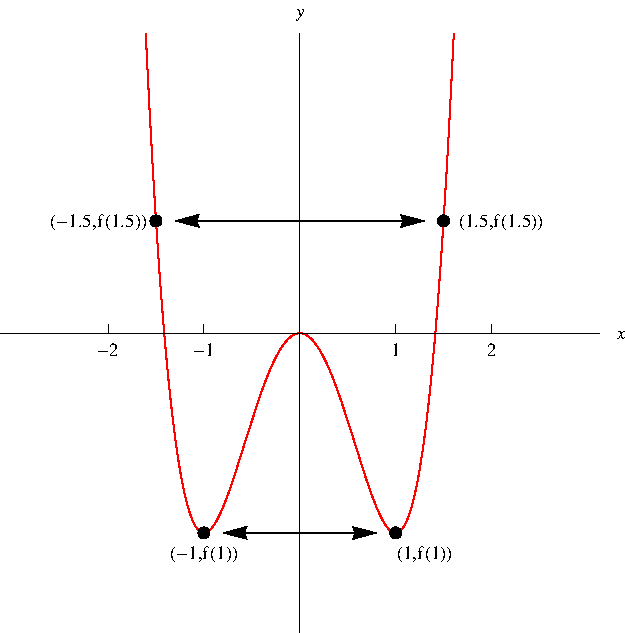
\includegraphics[height=5cm]{curve-sketching/pictures/01-01-even.pdf}%
%}}%
%\only<handout:2| 3>{%
%\ 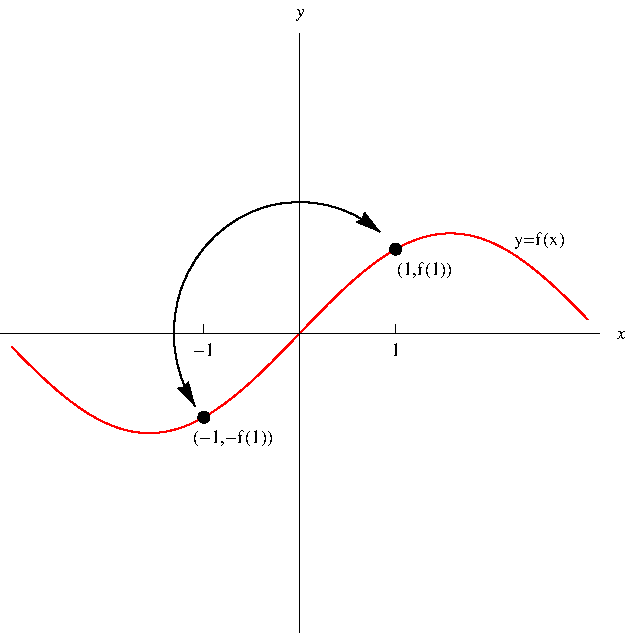
\includegraphics[height=5cm]{curve-sketching/pictures/01-01-odd.pdf}%
%}%
%\only<handout:3| 4->{%
%\ 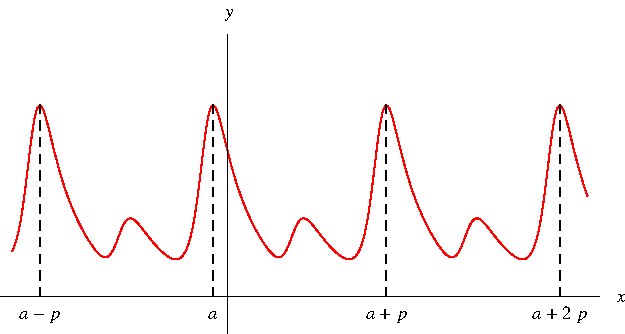
\includegraphics[height=5cm]{curve-sketching/pictures/04-05-periodic.pdf}%
%}
\end{center}
\end{frame}


\begin{frame}[t]
\begin{enumerate}
\setcounter{enumi}{4}
\item  Asymptotes
\end{enumerate}
\begin{itemize}
\item  \textbf{Horizontal asymptotes} can be found by finding $\lim\limits_{x\to\infty} f(x)$ and $\lim\limits_{x\to -\infty} f(x)$.
\item  If either of these equals a number $L$, then $y = L$ is a horizontal asymptote of $f$.  
\item  If neither limit exists, there is no horizontal asymptote.
\item  The line $x = a$ is a \textbf{Vertical asymptote} of $f$ if any of the following is true
\end{itemize}
\[
\begin{array}{ll}
\displaystyle \lim_{x\to a^+}f(x) = \infty &%
\displaystyle \lim_{x\to a^-}f(x) = \infty \\%
\displaystyle \lim_{x\to a^+}f(x) = -\infty &%
\displaystyle \lim_{x\to a^-}f(x) = -\infty %
\end{array}
\]
\begin{itemize}
\item  We may discuss slant asymptotes in another lecture if time allows.
\end{itemize}
\end{frame}


\begin{frame}[t]
\begin{enumerate}
\setcounter{enumi}{5}
\item  Intervals of increase or decrease
\end{enumerate}
\begin{itemize}
\item  To find intervals of increase or decrease, use the increasing/decreasing test.
\item  Compute $f'$.
\item  Find where $f'$ is positive or negative.
\item  Where $f'$ is positive, $f$ is increasing.
\item  Where $f'$ is negative, $f$ is decreasing.
\end{itemize}
\end{frame}




\begin{frame}[t]
\begin{enumerate}
\setcounter{enumi}{6}
\item  Local maxima and minima
\end{enumerate}
\begin{itemize}
\item  Find the critical numbers of $f$ (the numbers $c$ where $f'(c)$ doesn't exist or $f'(c) = 0$).
\item  Use the First Derivative Test on each of these numbers:
\item  If $f'$ changes from positive to negative at a critical number $c$, then $c$ is a local maximum.
\item  If $f'$ changes from negative to positive at a critical number $c$, then $c$ is a local minimum.
\item  If $f'$ doesn't change sign at a critical number $c$, then $c$ is neither a local maximum nor a local minimum.
\end{itemize}
\end{frame}



\begin{frame}[t]
\begin{enumerate}
\setcounter{enumi}{7}
\item  Concavity and points of inflection
\end{enumerate}
\begin{itemize}
\item  To find inflection points and intervals of concavity, use the concavity test.
\item  Compute $f''$.
\item  Find where $f''$ is positive or negative.
\item  Where $f''$ is positive, $f$ is concave up.
\item  Where $f''$ is negative, $f$ is concave down.
\item  Inflection points occur when $f''$ changes signs.
\end{itemize}
\end{frame}
% end module curve-sketching-guidelines

%% begin module curve-sketching-guidelines-ex1
\begin{frame}[t]
\begin{example} %[Example 1, p. 245]
\begin{columns}[t]
\column{.45\textwidth}
Sketch the curve $y = \frac{2x^2}{\alertNoH{ 3}{x^2-1}}$.
%\ 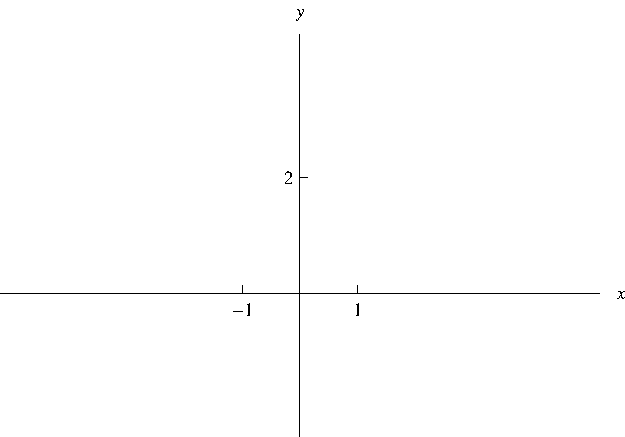
\includegraphics[width=5cm]{curve-sketching/pictures/04-05-ex1a.pdf}%
\psset{xunit=0.25cm, yunit=0.25cm}
\begin{pspicture}(-10,-5.5)(10.5,9)
\psframe*[linecolor=white](-10,-5.5)(10.5,9)
\tiny
\psaxes[ticks=none, labels=none]{<->}(0,0)(-10,-5.5)(10,8.5)
\psline[linecolor=red!1](1,9)(1,9.001)
\psline[linecolor=red!1](1,-5.2)(1,-5.201)

\fcLabels{10}{8.5}
\fcXTickWithLabel{1}{$1$}
\fcXTickWithLabel{-1}{$-1$}
\fcYTickWithLabel{2}{$2$}
\psline[linecolor=red!1](1,9)(1,9.001)
%Function formula: \frac{2 x^{2}}{x^{2}-1}
%\psplot[linecolor=\fcColorGraph, plotpoints=1000]{1.15}{9.9}{x 2 exp 2 mul -1 x 2 exp add div }
%\psplot[linecolor=\fcColorGraph, plotpoints=1000]{-0.85}{0.85}{x 2 exp 2 mul -1 x 2 exp add div }
%\psplot[linecolor=\fcColorGraph, plotpoints=1000]{-9.9}{-1.15}{x 2 exp 2 mul -1 x 2 exp add div }
\end{pspicture}

\invisible<1->{
\abovedisplayskip=0pt
\belowdisplayskip=0pt
\[
\begin{array}{|@{}c@{}|c@{}|c@{}|}
\hline
\textrm{Interval}&\textrm{I/D}&\textrm{Concavity}\\
\hline
(-\infty , -1)&%
\textrm{I}&\\%
(-1 , 0)&%
\textrm{D}&\\%
(0 , 1)&%
\textrm{D}&\\%
(1 , \infty)&%
\textrm{I}&\\%
\hline
\end{array}
\]
}
\column{.55\textwidth}
\begin{enumerate}
\item<2->  Domain
\end{enumerate}
\uncover<2->{%
The domain of the function is \uncover<3->{\alertNoH{ 3}{$(-\infty , -1) \cup (-1, 1)\cup (1,\infty )$}.}
}%
\end{columns}
\end{example}
\end{frame}


\begin{frame}[t]
\begin{example} %[Example 1, p. 245]
\begin{columns}[t]
\column{.45\textwidth}
Sketch the curve $y = \frac{2x^2}{x^2-1}$.
\psset{xunit=0.25cm, yunit=0.25cm}
\begin{pspicture}(-10,-5.5)(10.5,9)
\psframe*[linecolor=white](-10,-5.5)(10.5,9)
\tiny
\psaxes[ticks=none, labels=none]{<->}(0,0)(-10,-5.5)(10,8.5)
\psline[linecolor=red!1](1,9)(1,9.001)
\psline[linecolor=red!1](1,-5.2)(1,-5.201)

\fcLabels{10}{8.5}
\fcXTickWithLabel{1}{$1$}
\fcXTickWithLabel{-1}{$-1$}
\fcYTickWithLabel{2}{$2$}
\uncover<7->{
\fcFullDot{0}{0}
}
\end{pspicture}
%\ \only<handout:0| -5>{%
%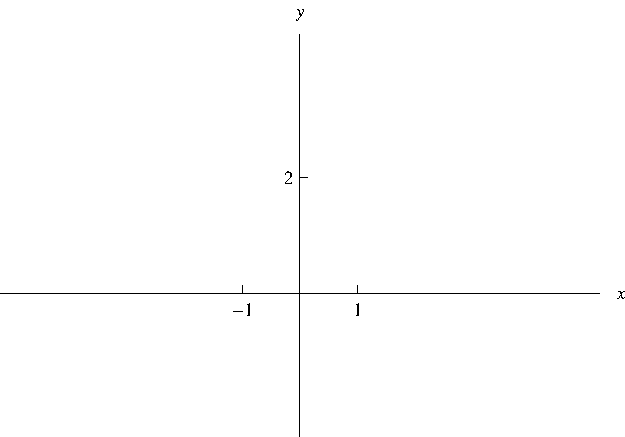
\includegraphics[width=5cm]{curve-sketching/pictures/04-05-ex1a.pdf}%
%}%
%\only<6->{%
%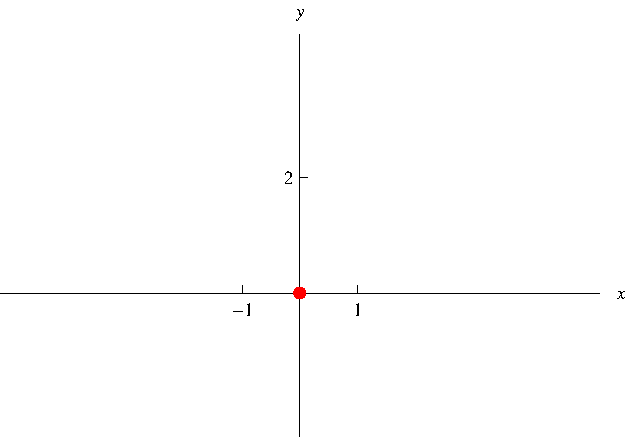
\includegraphics[width=5cm]{curve-sketching/pictures/04-05-ex1b.pdf}%
%}%

\invisible<1->{
\abovedisplayskip=0pt
\belowdisplayskip=0pt
\[
\begin{array}{|@{}c@{}|c@{}|c@{}|}
\hline
\textrm{Interval}&\textrm{I/D}&\textrm{Concavity}\\
\hline
(-\infty , -1)&%
\textrm{I}&\\%
(-1 , 0)&%
\textrm{D}&\\%
(0 , 1)&%
\textrm{D}&\\%
(1 , \infty)&%
\textrm{I}&\\%
\hline
\end{array}
\]
}
\column{.55\textwidth}
\begin{enumerate}
\setcounter{enumi}{2}
\item  Intercepts
\end{enumerate}
\begin{itemize}
\item<2-| alert@2-3>  $y$-intercept: $f(0) = $ \uncover<3->{$0$.}
\item<2-| alert@4-5>  $x$-intercept: $f(x) = 0$ when $x = $ \uncover<5->{$0$.}
\item<6->  The only intercept is $\alertNoH{7}{(0,0)}$.
\end{itemize}
\end{columns}
\end{example}
\end{frame}


\begin{frame}[t]
\begin{example} %[Example 1, p. 245]
\begin{columns}[t]
\column{.45\textwidth}
Sketch the curve $y = \frac{2x^2}{x^2-1}$.
\psset{xunit=0.25cm, yunit=0.25cm}
\begin{pspicture}(-10,-5.5)(10.5,9)
\psframe*[linecolor=white](-10,-5.5)(10.5,9)
\tiny
\psaxes[ticks=none, labels=none]{<->}(0,0)(-10,-5.5)(10,8.5)
\psline[linecolor=red!1](1,9)(1,9.001)
\psline[linecolor=red!1](1,-5.2)(1,-5.201)

\fcLabels{10}{8.5}
\fcXTickWithLabel{1}{$1$}
\fcXTickWithLabel{-1}{$-1$}
\fcYTickWithLabel{2}{$2$}
\fcFullDot{0}{0}
\end{pspicture}

%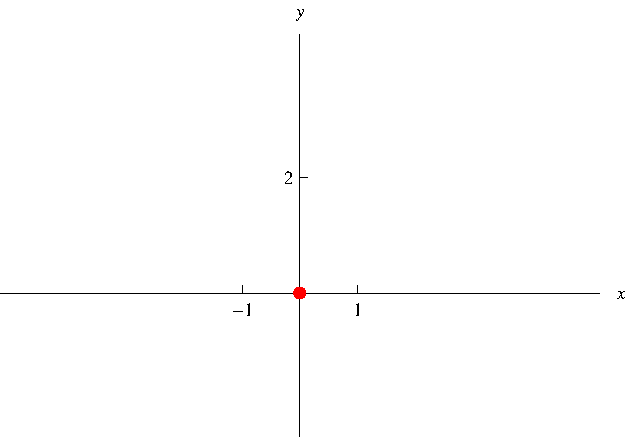
\includegraphics[width=5cm]{curve-sketching/pictures/04-05-ex1b.pdf}%

\invisible<1->{
\abovedisplayskip=0pt
\belowdisplayskip=0pt
\[
\begin{array}{|@{}c@{}|c@{}|c@{}|}
\hline
\textrm{Interval}&\textrm{I/D}&\textrm{Concavity}\\
\hline
(-\infty , -1)&%
\textrm{I}&\\%
(-1 , 0)&%
\textrm{D}&\\%
(0 , 1)&%
\textrm{D}&\\%
(1 , \infty)&%
\textrm{I}&\\%
\hline
\end{array}
\]
}
\column{.55\textwidth}
\begin{enumerate}
\setcounter{enumi}{3}
\item  Symmetry
\end{enumerate}
\[
\uncover<2->{%
f(-x) = \alertNoH{ 3-4}{\frac{2(-x)^2}{(-x)^2-1}} %
}%
\uncover<3->{%
\alertNoH{ 3-4}{ = \uncover<4->{\frac{2x^2}{x^2-1}}} %
}%
\uncover<5->{%
 = f(x)
}%
\]
\uncover<6->{Therefore $f$ is \uncover<7->{\alertNoH{ 7}{even}.}}
\end{columns}
\end{example}
\end{frame}


\begin{frame}[t]
\begin{example} %[Example 1, p. 245]
\begin{columns}[t]
\column{.45\textwidth}
Sketch the curve $y = \frac{2x^2}{x^2-1}$.
\psset{xunit=0.25cm, yunit=0.25cm}
\begin{pspicture}(-10,-5.5)(10.5,9)
\psframe*[linecolor=white](-10,-5.5)(10.5,9)
\tiny
\psaxes[ticks=none, labels=none]{<->}(0,0)(-10,-5.5)(10,8.5)
\psline[linecolor=red!1](1,9)(1,9.001)
\psline[linecolor=red!1](1,-5.2)(1,-5.201)

\fcLabels{10}{8.5}
\uncover<1-14>{
\fcXTickWithLabel{1}{$1$}
\fcXTickWithLabel{-1}{$-1$}
}
\uncover<1-4>{
\fcYTickWithLabel{2}{$2$}
}
\fcFullDot{0}{0}
\uncover<5->{
\psline[linestyle=dashed, linewidth=0.3pt](-9.97,2 )(9.97,2)
\rput[t](-8.5, 1.9){$y=2$}
}
\uncover<4->{ %
\psplot[arrows=->,linecolor=\fcColorGraph, plotpoints=1000]{8}{9.9}{x 2 exp 2 mul -1 x 2 exp add div }
} %
\uncover<8->{ %
\psplot[arrows=<-,linecolor=\fcColorGraph, plotpoints=1000]{1.2}{1.8}{x 2 exp 2 mul -1 x 2 exp add div }
} %
\uncover<10->{
\psplot[arrows=->, linecolor=\fcColorGraph, plotpoints=1000]{0.65}{0.8}{x 2 exp 2 mul -1 x 2 exp add div }
}
\uncover<12->{
\psplot[arrows=<-, linecolor=\fcColorGraph, plotpoints=1000]{-0.8}{-0.65}{x 2 exp 2 mul -1 x 2 exp add div }
}

\uncover<4->{ %
\psplot[arrows=<-, linecolor=\fcColorGraph, plotpoints=1000]{-9.9}{-8}{x 2 exp 2 mul -1 x 2 exp add div }
} %
\uncover<14->{ %
\psplot[arrows=->, linecolor=\fcColorGraph, plotpoints=1000]{-1.8}{-1.2}{x 2 exp 2 mul -1 x 2 exp add div }
} %
\uncover<15->{ %
\psline[linestyle=dashed, linewidth=0.3pt](-1,-5)(-1,8)
\rput[r](-1.4, -3.5){$x=-1$}
\psline[linestyle=dashed, linewidth=0.3pt](1,-5)(1,8)
\rput[l](1.4, -3.5){$x=1$}
} %
\end{pspicture}

%\ \only<handout:0| -3>{%
%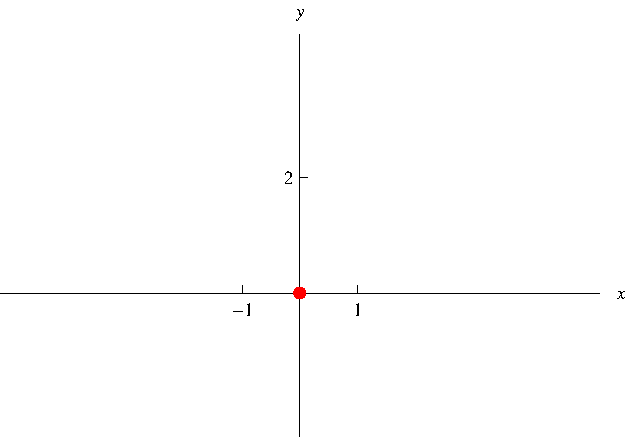
\includegraphics[width=5cm]{curve-sketching/pictures/04-05-ex1b.pdf}%
%}%
%\only<handout:0| 4>{%
%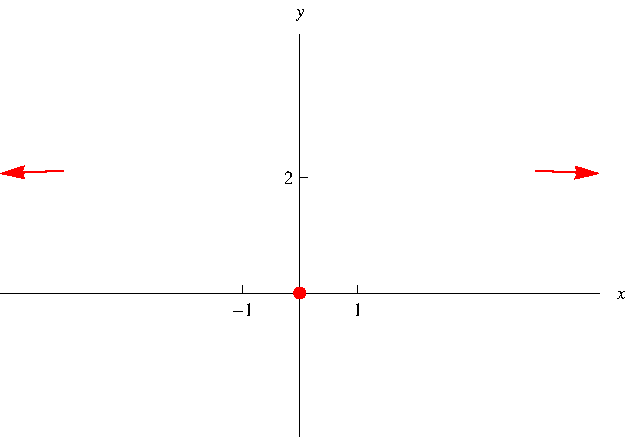
\includegraphics[width=5cm]{curve-sketching/pictures/04-05-ex1c.pdf}%
%}%
%\only<handout:0| 5-7>{%
%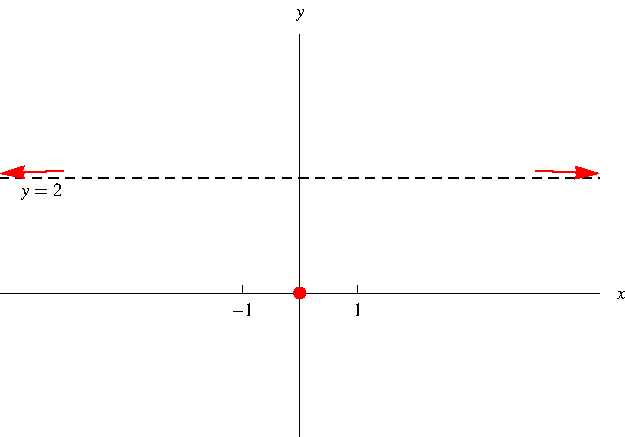
\includegraphics[width=5cm]{curve-sketching/pictures/04-05-ex1d.pdf}%
%}%
%\only<handout:0| 8-9>{%
%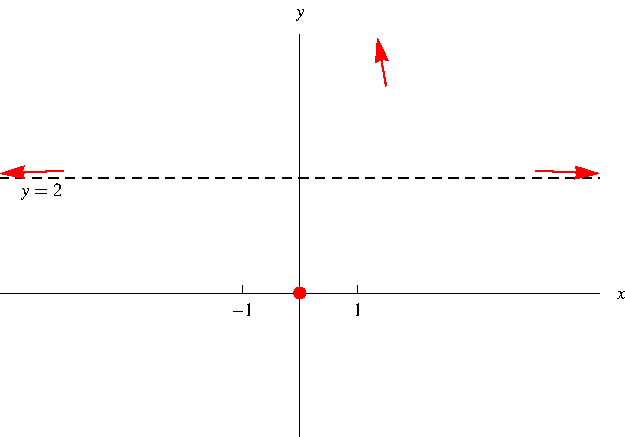
\includegraphics[width=5cm]{curve-sketching/pictures/04-05-ex1e.pdf}%
%}%
%\only<handout:0| 10-11>{%
%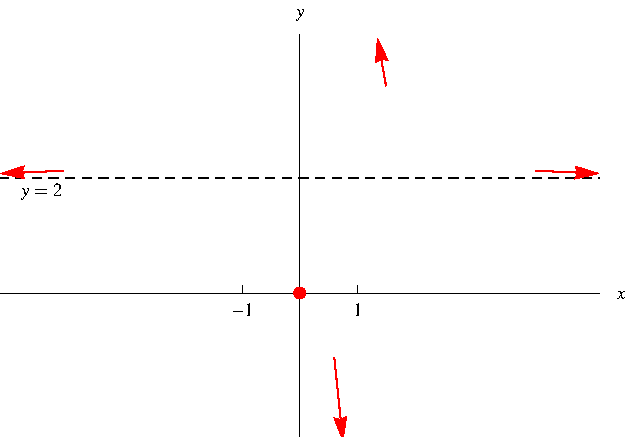
\includegraphics[width=5cm]{curve-sketching/pictures/04-05-ex1f.pdf}%
%}%
%\only<handout:0| 12-13>{%
%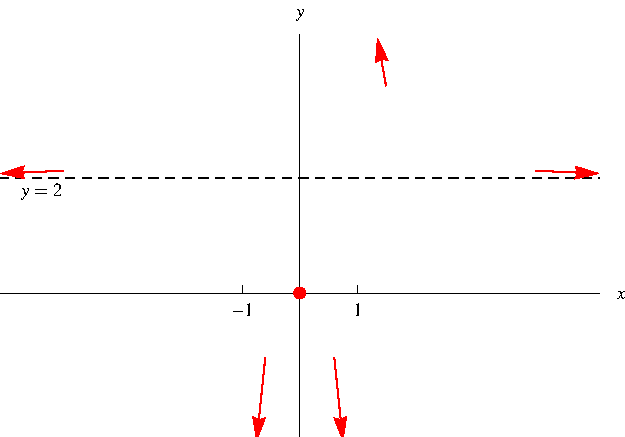
\includegraphics[width=5cm]{curve-sketching/pictures/04-05-ex1g.pdf}%
%}%
%\only<handout:0| 14>{%
%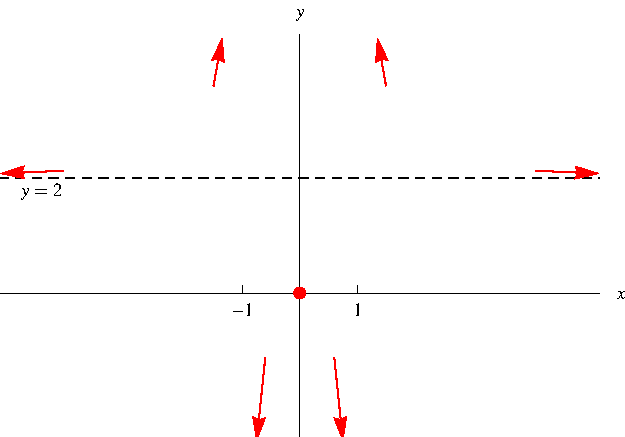
\includegraphics[width=5cm]{curve-sketching/pictures/04-05-ex1h.pdf}%
%}%
%\only<15->{%
%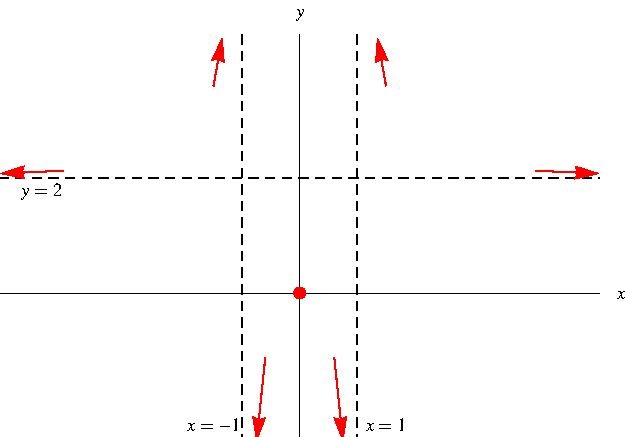
\includegraphics[width=5cm]{curve-sketching/pictures/04-05-ex1i.pdf}%
%}%

\invisible<1->{
\abovedisplayskip=0pt
\belowdisplayskip=0pt
\[
\begin{array}{|@{}c@{}|c@{}|c@{}|}
\hline
\textrm{Interval}&\textrm{I/D}&\textrm{Concavity}\\
\hline
(-\infty , -1)&%
\textrm{I}&\\%
(-1 , 0)&%
\textrm{D}&\\%
(0 , 1)&%
\textrm{D}&\\%
(1 , \infty)&%
\textrm{I}&\\%
\hline
\end{array}
\]
}

\column{.55\textwidth}
\begin{enumerate}
\setcounter{enumi}{4}
\item  Asymptotes
\end{enumerate}
\abovedisplayskip=0pt
\belowdisplayskip=0pt
\[
\uncover<2->{%
\lim_{x\to\pm\infty}\frac{2x^2}{x^2-1}%
}%
\uncover<3->{%
 = \lim_{x\to\pm\infty}\frac{2}{1 - 1/x^2}%
}%
\uncover<4->{%
 = 2%
}%
\]
\uncover<5->{$y = 2$ is a horizontal asymptote.}
\uncover<6->{%
\abovedisplayskip=0pt
\belowdisplayskip=0pt
\[
\begin{array}{r@{}c@{}l}
\displaystyle \alertNoH{ 7-8}{\lim_{x\to 1^+}\frac{2x^2}{x^2-1}} & \alertNoH{ 7-8}{=} & \uncover<8->{\alertNoH{ 8}{\infty}} \\%
\displaystyle \alertNoH{ 9-10}{\lim_{x\to 1^-}\frac{2x^2}{x^2-1}} & \alertNoH{ 9-10}{=} & \uncover<10->{\alertNoH{ 10}{-\infty}} \\%
\displaystyle \alertNoH{ 11-12}{\lim_{x\to -1^+}\frac{2x^2}{x^2-1}} & \alertNoH{ 11-12}{=} & \uncover<12->{\alertNoH{ 12}{-\infty}} \\%
\displaystyle \alertNoH{ 13-14}{\lim_{x\to -1^-}\frac{2x^2}{x^2-1}} & \alertNoH{ 13-14}{=} & \uncover<14->{\alertNoH{ 14}{\infty}} %
\end{array}
\]
}%
\uncover<15->{%
$x = \pm 1$ are vertical asymptotes.%
}%
\end{columns}
\end{example}
\end{frame}


\begin{frame}[t]
\begin{example} %[Example 1, p. 245]
\begin{columns}[t]
\column{.45\textwidth}
Sketch the curve $y = \frac{2x^2}{x^2-1}$.
\psset{xunit=0.25cm, yunit=0.25cm}
\begin{pspicture}(-10,-5.5)(10.5,9)
\psframe*[linecolor=white](-10,-5.5)(10.5,9)
\tiny
\psaxes[ticks=none, labels=none]{<->}(0,0)(-10,-5.5)(10,8.5)
\psline[linecolor=red!1](1,9)(1,9.001)
\psline[linecolor=red!1](1,-5.2)(1,-5.201)

\fcLabels{10}{8.5}
\fcFullDot{0}{0}
\psline[linestyle=dashed, linewidth=0.3pt](-9.97,2 )(9.97,2)
\rput[t](-8.5, 1.9){$y=2$}
\psplot[arrows=->,linecolor=\fcColorGraph, plotpoints=1000]{8}{9.9}{x 2 exp 2 mul -1 x 2 exp add div }
\psplot[arrows=<-,linecolor=\fcColorGraph, plotpoints=1000]{1.2}{1.8}{x 2 exp 2 mul -1 x 2 exp add div }
\psplot[arrows=->, linecolor=\fcColorGraph, plotpoints=1000]{0.65}{0.8}{x 2 exp 2 mul -1 x 2 exp add div }
\psplot[arrows=<-, linecolor=\fcColorGraph, plotpoints=1000]{-0.8}{-0.65}{x 2 exp 2 mul -1 x 2 exp add div }
\psplot[arrows=<-, linecolor=\fcColorGraph, plotpoints=1000]{-9.9}{-8}{x 2 exp 2 mul -1 x 2 exp add div }
\psplot[arrows=->, linecolor=\fcColorGraph, plotpoints=1000]{-1.8}{-1.2}{x 2 exp 2 mul -1 x 2 exp add div }
\psline[linestyle=dashed, linewidth=0.3pt](-1,-5)(-1,8)
\rput[r](-1.4, -3.5){$x=-1$}
\psline[linestyle=dashed, linewidth=0.3pt](1,-5)(1,8)
\rput[l](1.4, -3.5){$x=1$}
\end{pspicture}

%\ \only<1->{%
%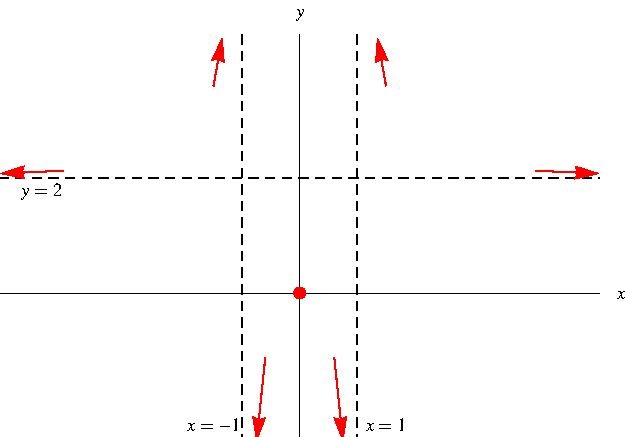
\includegraphics[width=5cm]{curve-sketching/pictures/04-05-ex1i.pdf}%
%}%

\abovedisplayskip=0pt
\belowdisplayskip=0pt
\[
\begin{array}{|@{}c@{}|c@{}|c@{}|}
\hline
\textrm{Interval}&\alertNoH{ 12}{\textrm{I/D}}&\textrm{Concavity}\\
\hline
(-\infty , -1)&%
\uncover<12->{\alertNoH{ 12}{\textrm{I}}}&\\%
(-1 , 0)&%
\uncover<12->{\alertNoH{ 12}{\textrm{I}}}&\\%
(0 , 1)&%
\uncover<12->{\alertNoH{ 12}{\textrm{D}}}&\\%
(1 , \infty)&%
\uncover<12->{\alertNoH{ 12}{\textrm{D}}}&\\%
\hline
\end{array}
\]

\column{.55\textwidth}
\begin{enumerate}
\setcounter{enumi}{5}
\item  Intervals of increase or decrease
\end{enumerate}
\abovedisplayskip=0pt
\belowdisplayskip=0pt
\begin{eqnarray*}
\uncover<2->{%
\alertNoH{ 3-4}{f'(x)}%
}%
& \uncover<2->{\alertNoH{ 3-4}{ = }} &%
\uncover<4->{%
\alertNoH{ 4}{\frac{(x^2-1)(4x) - 2x^2(2x)}{(x^2-1)^2}}%
}\\%
&\uncover<5->{ = } &%
\uncover<5->{%
 \frac{-4x}{(x^2-1)^2}%
}%
\end{eqnarray*}
\uncover<6->{%
\[
\begin{array}{|c@{}|c@{}|c@{}|c@{}|}
\hline
& \alertNoH{ 7-8}{-4x} & \alertNoH{ 9-10}{(x^2-1)^2} & \alertNoH{ 11}{f'} \\
\hline
(-\infty , -1) & \alertNoH{ 7-8}{\uncover<8->{+}} & \alertNoH{ 9-10}{\uncover<10->{+}} & \alertNoH{ 11}{\uncover<11->{+}} \\
(-1 , 0) & \alertNoH{ 7-8}{\uncover<8->{+}} & \alertNoH{ 9-10}{\uncover<10->{+}} & \alertNoH{ 11}{\uncover<11->{+}} \\
(0 , 1) & \alertNoH{ 7-8}{\uncover<8->{-}} & \alertNoH{ 9-10}{\uncover<10->{+}} & \alertNoH{ 11}{\uncover<11->{-}} \\
(1 , \infty) & \alertNoH{ 7-8}{\uncover<8->{-}} & \alertNoH{ 9-10}{\uncover<10->{+}} & \alertNoH{ 11}{\uncover<11->{-}} \\
\hline
\end{array}
\]
}%
\end{columns}
\end{example}
\end{frame}


\begin{frame}[t]
\begin{example} %[Example 1, p. 245]
\begin{columns}[t]
\column{.45\textwidth}
Sketch the curve $y = \frac{2x^2}{x^2-1}$.
\psset{xunit=0.25cm, yunit=0.25cm}
\begin{pspicture}(-10,-5.5)(10.5,9)
\psframe*[linecolor=white](-10,-5.5)(10.5,9)
\tiny
\psaxes[ticks=none, labels=none]{<->}(0,0)(-10,-5.5)(10,8.5)
\psline[linecolor=red!1](1,9)(1,9.001)
\psline[linecolor=red!1](1,-5.2)(1,-5.201)

\fcLabels{10}{8.5}
\fcFullDot{0}{0}
\psline[linestyle=dashed, linewidth=0.3pt](-9.97,2 )(9.97,2)
\rput[t](-8.5, 1.9){$y=2$}
\psplot[arrows=->,linecolor=\fcColorGraph, plotpoints=1000]{8}{9.9}{x 2 exp 2 mul -1 x 2 exp add div }
\psplot[arrows=<-,linecolor=\fcColorGraph, plotpoints=1000]{1.2}{1.8}{x 2 exp 2 mul -1 x 2 exp add div }
\psplot[arrows=->, linecolor=\fcColorGraph, plotpoints=1000]{0.65}{0.8}{x 2 exp 2 mul -1 x 2 exp add div }
\psplot[arrows=<-, linecolor=\fcColorGraph, plotpoints=1000]{-0.8}{-0.65}{x 2 exp 2 mul -1 x 2 exp add div }
\psplot[arrows=<-, linecolor=\fcColorGraph, plotpoints=1000]{-9.9}{-8}{x 2 exp 2 mul -1 x 2 exp add div }
\psplot[arrows=->, linecolor=\fcColorGraph, plotpoints=1000]{-1.8}{-1.2}{x 2 exp 2 mul -1 x 2 exp add div }
\psline[linestyle=dashed, linewidth=0.3pt](-1,-5)(-1,8)
\rput[r](-1.4, -3.5){$x=-1$}
\psline[linestyle=dashed, linewidth=0.3pt](1,-5)(1,8)
\rput[l](1.4, -3.5){$x=1$}
\end{pspicture}

%\ \only<1->{%
%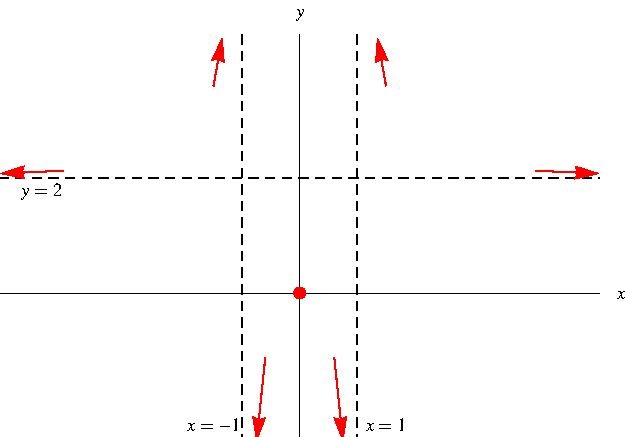
\includegraphics[width=5cm]{curve-sketching/pictures/04-05-ex1i.pdf}%
%}%

\abovedisplayskip=0pt
\belowdisplayskip=0pt
\[
\begin{array}{|@{}c@{}|c@{}|c@{}|}
\hline
\textrm{Interval}&\textrm{I/D}&\textrm{Concavity}\\
\hline
(-\infty , -1)&%
\textrm{I}&\\%
(-1 , 0)&%
\textrm{I}&\\%
(0 , 1)&%
\textrm{D}&\\%
(1 , \infty)&%
\textrm{D}&\\%
\hline
\end{array}
\]

\column{.55\textwidth}
\begin{enumerate}
\setcounter{enumi}{6}
\item  Local maxima and minima
\end{enumerate}
\[
\begin{array}{|c@{}|c@{}|c@{}|c@{}|}
\hline
& -4x & (x^2-1)^2 & f' \\
\hline
(-\infty , -1) & + & + & + \\
\alertNoH{ 2}{(-1 , 0)} & + & + & \alertNoH{ 2}{+} \\
\alertNoH{ 2}{(0 , 1)} & - & + & \alertNoH{ 2}{-} \\
(1 , \infty) & - & + & - \\
\hline
\end{array}
\]
\begin{itemize}
\item<2->  $f'$ changes sign from $+$ to $-$ at $0$.
\item<3->  Therefore $(0,0)$ is a local maximum.
\end{itemize}
\end{columns}
\end{example}
\end{frame}

\begin{frame}[t]
\begin{example} %[Example 1, p. 245]
\begin{columns}[t]
\column{.45\textwidth}
Sketch the curve $y = \frac{2x^2}{x^2-1}$.
\psset{xunit=0.25cm, yunit=0.25cm}
\begin{pspicture}(-10,-5.5)(10.5,9)
\psframe*[linecolor=white](-10,-5.5)(10.5,9)
\tiny
\psaxes[ticks=none, labels=none]{<->}(0,0)(-10,-5.5)(10,8.5)
\psline[linecolor=red!1](1,9)(1,9.001)
\psline[linecolor=red!1](1,-5.2)(1,-5.201)

\fcLabels{10}{8.5}
\fcFullDot{0}{0}
\psline[linestyle=dashed, linewidth=0.3pt](-9.97,2 )(9.97,2)
\rput[t](-8.5, 1.9){$y=2$}
\psline[linestyle=dashed, linewidth=0.3pt](-1,-5)(-1,8)
\rput[r](-1.4, -3.5){$x=-1$}
\psline[linestyle=dashed, linewidth=0.3pt](1,-5)(1,8)
\rput[l](1.4, -3.5){$x=1$}
\uncover<1-13>{ %
\psplot[arrows=->,linecolor=\fcColorGraph, plotpoints=1000]{8}{9.9}{x 2 exp 2 mul -1 x 2 exp add div }
\psplot[arrows=<-,linecolor=\fcColorGraph, plotpoints=1000]{1.2}{1.8}{x 2 exp 2 mul -1 x 2 exp add div }
\psplot[arrows=->, linecolor=\fcColorGraph, plotpoints=1000]{0.65}{0.8}{x 2 exp 2 mul -1 x 2 exp add div }
\psplot[arrows=<-, linecolor=\fcColorGraph, plotpoints=1000]{-0.8}{-0.65}{x 2 exp 2 mul -1 x 2 exp add div }
\psplot[arrows=<-, linecolor=\fcColorGraph, plotpoints=1000]{-9.9}{-8}{x 2 exp 2 mul -1 x 2 exp add div }
\psplot[arrows=->, linecolor=\fcColorGraph, plotpoints=1000]{-1.8}{-1.2}{x 2 exp 2 mul -1 x 2 exp add div }
}
\uncover<14->{ %
\psplot[linecolor=\fcColorGraph, plotpoints=1000]{1.15}{9.9}{x 2 exp 2 mul -1 x 2 exp add div }
\psplot[linecolor=\fcColorGraph, plotpoints=1000]{-0.85}{0.85}{x 2 exp 2 mul -1 x 2 exp add div }
\psplot[linecolor=\fcColorGraph, plotpoints=1000]{-9.9}{-1.15}{x 2 exp 2 mul -1 x 2 exp add div }
} %
\end{pspicture}
%\ \only<handout:0| -13>{%
%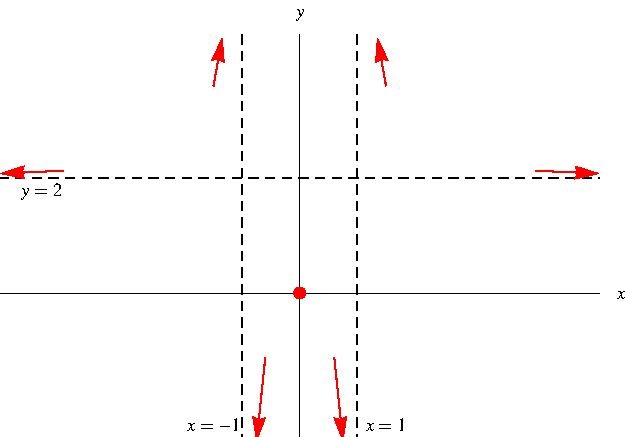
\includegraphics[width=5cm]{curve-sketching/pictures/04-05-ex1i.pdf}%
%}%
%\only<14->{%
%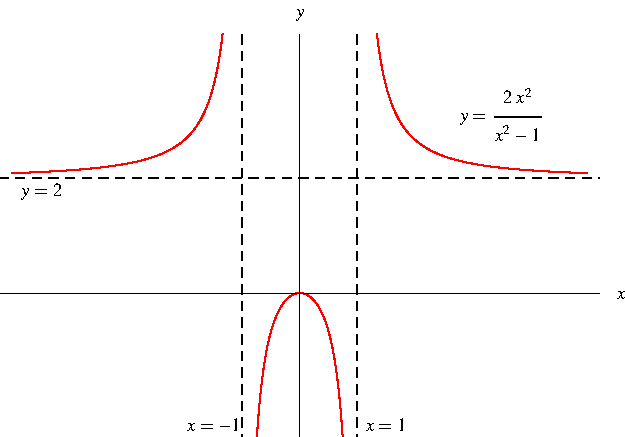
\includegraphics[width=5cm]{curve-sketching/pictures/04-05-ex1j.pdf}%
%}%

\abovedisplayskip=0pt
\belowdisplayskip=0pt
\[
\begin{array}{|@{}c@{}|c@{}|c@{}|}
\hline
\textrm{Interval}&\textrm{I/D}&\alertNoH{ 12}{\textrm{Concavity}}\\
\hline
(-\infty , -1)&%
\textrm{I}&\uncover<12->{\alertNoH{ 12}{\textrm{up}}}\\%
(-1 , 0)&%
\textrm{I}&\uncover<12->{\alertNoH{ 12}{\textrm{down}}}\\%
(0 , 1)&%
\textrm{D}&\uncover<12->{\alertNoH{ 12}{\textrm{down}}}\\%
(1 , \infty)&%
\textrm{D}&\uncover<12->{\alertNoH{ 12}{\textrm{up}}}\\%
\hline
\end{array}
\]

\column{.55\textwidth}
\begin{enumerate}
\setcounter{enumi}{7}
\item  Concavity and points of inflection
\end{enumerate}
\abovedisplayskip=0pt
\belowdisplayskip=0pt
\begin{eqnarray*}
& & \uncover<2->{%
\ \ \alertNoH{ 3-4}{f''(x)}%
}\\%
%& \uncover<2->{\alertNoH{ 3-4}{ = }} &%
&&\uncover<4->{%
\alertNoH{ 4}{ = \frac{-4(x^2-1)^2+4x\cdot 2(x^2-1)2x}{(x^2-1)^4}}%
}\\%
%&\uncover<5->{ = } &%
&&\uncover<5->{%
 =  \frac{12x^2+4}{(x^2-1)^3}%
}%
\end{eqnarray*}
\uncover<6->{%
\[
\begin{array}{|@{}c@{}|c@{}|c@{}|c@{}|}
\hline
& \alertNoH{ 7-8}{12x^2+4} & \alertNoH{ 9-10}{(x^2-1)^3} & \alertNoH{ 11}{f''} \\
\hline
(-\infty , -1) & \alertNoH{ 7-8}{\uncover<8->{+}} & \alertNoH{ 9-10}{\uncover<10->{+}} & \alertNoH{ 11}{\uncover<11->{+}} \\
(-1 , 1) & \alertNoH{ 7-8}{\uncover<8->{+}} & \alertNoH{ 9-10}{\uncover<10->{-}} & \alertNoH{ 11}{\uncover<11->{-}} \\
(1 , \infty) & \alertNoH{ 7-8}{\uncover<8->{+}} & \alertNoH{ 9-10}{\uncover<10->{+}} & \alertNoH{ 11}{\uncover<11->{+}} \\
\hline
\end{array}
\]
}%
\uncover<13,14->{%
No points of inflection because $\pm 1$ are not in the domain of $f$.
}%
\end{columns}
\end{example}
\end{frame}
% end module curve-sketching-guidelines-ex1

%% begin module EVT-statement
\begin{frame}[t]
\begin{theorem}[The Extreme Value Theorem]
If $f$ is continuous on a closed interval $[a,b]$, then $f$ attains its absolute maximum value $f(c)$ and its absolute minimum value $f(d)$ at some numbers $c$ and $d$ in $[a,b]$.
\end{theorem}
\begin{columns}[c]
\column{.3\textwidth}
\ \uncover<2->{%
\psset{xunit=0.6cm, yunit=0.6cm}
\begin{pspicture}(-5, -5)(5,5) 
\psframe*[linecolor=white](-5,-5)(5,5) 
\psaxes[ticks=none, labels=none]{<->}(0,0)(-0.5,-0.8)(5.2,3.2)\tiny
\psLabels{5.2}{3.2}
%Function formula: (-3/4+1/2 (x))^{2}+1 
\psplot[linecolor=red, plotpoints=1000]{0.5}{4}{1 x 0.5 mul -0.75 add 2 exp add }
\psFullDot{0.5}{1.25}
\psFullDot{4}{2.5625}
\psline[linestyle=dashed](1.5,0)(1.5,1)
\psline[linestyle=dashed](4,0)(4,2.5625)
\psXTick{0.5}
\rput[t](0.5, -0.2){$a$}
\psXTick{1.5}
\rput[t](1.5, -0.2){$d$}
\psXTick{4}
\rput[t](4, -0.2){$c=b$}
\end{pspicture} 
%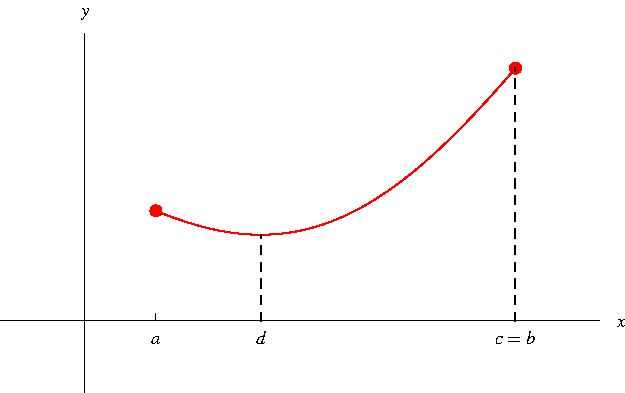
\includegraphics[width=4cm]{maxima-minima/pictures/04-01-evtb.pdf}%
}%
\column{.3\textwidth}
\psset{xunit=0.6cm, yunit=0.6cm}
\begin{pspicture}(-5, -5)(5,5) 
\psframe*[linecolor=white](-5,-5)(5,5) 
\psaxes[ticks=none, labels=none]{<->}(0,0)(-0.5,-0.8)(5.2,3.2)\tiny
\psLabels{5.2}{3.2}
%Function formula: 1/2+3 (x)+1/6 ((x)^{3})-11/8 ((x)^{2}) 
\psplot[linecolor=red, plotpoints=1000]{0.5}{4.8}{x 2 exp -1.375 mul x 3 exp 0.166667 mul x 3 mul 0.5 add add add }
\psFullDot{0.5}{1.67708}
\psFullDot{4.8}{1.652}
\psline[linestyle=dashed](1.5,0)(1.5,2.46875)
\psline[linestyle=dashed](4,0)(4,1.16667)
\psXTick{0.5}
\rput[t](0.5, -0.2){$a$}
\psXTick{1.5}
\rput[t](1.5, -0.2){$c$}
\psXTick{4}
\rput[t](4, -0.2){$d$}
\psXTick{4.8}
\rput[t](4.8, -0.2){$b$}
\end{pspicture} 
%\ 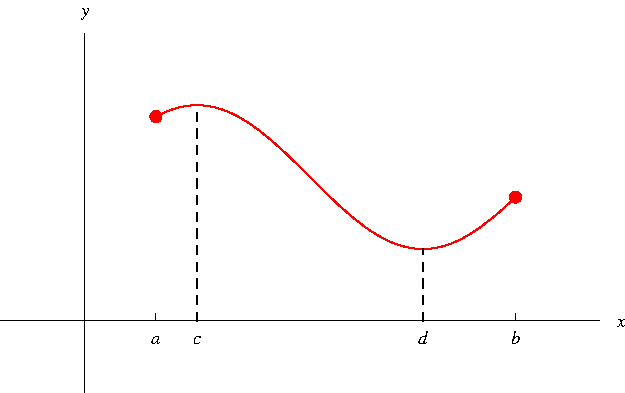
\includegraphics[width=4cm]{maxima-minima/pictures/04-01-evta.pdf}%
\column{.3\textwidth}
\ \uncover<3->{%
\psset{xunit=0.6cm, yunit=0.6cm}
\begin{pspicture}(-5, -5)(5,5) 
\psframe*[linecolor=white](-5,-5)(5,5) 
\psaxes[ticks=none, labels=none]{<->}(0,0)(-0.5,-0.8)(5.2,3.2)\tiny
\psLabels{5.2}{3.2}
%Function formula: -3/2+10 (x)+5/2 ((x)^{3})-1/4 ((x)^{4})-33/4 ((x)^{2}) 
\psplot[linecolor=red, plotpoints=1000]{0.5}{4.5}{x 2 exp -8.25 mul x 4 exp -0.25 mul x 3 exp 2.5 mul x 10 mul -1.5 add add add add }
\psline[linestyle=dashed](1,0)(1,2.5)
\psline[linestyle=dashed](2.5,0)(2.5,1.23438)
\psline[linestyle=dashed](4,0)(4,2.5)

\psFullDot{0.5}{1.73438}
\psXTick{0.5}
\rput[t](0.5, -0.2){$a$}

\psXTick{1}
\rput[t](1, -0.2){$c_1$}

\psXTick{4}
\rput[t](4, -0.2){$c_2$}

\psXTick{2.5}
\rput[t](2.5, -0.2){$d$}

\psXTick{4.5}
\psFullDot{4.5}{1.73438}
\rput[t](4.5, -0.2){$b$}
\end{pspicture} 
%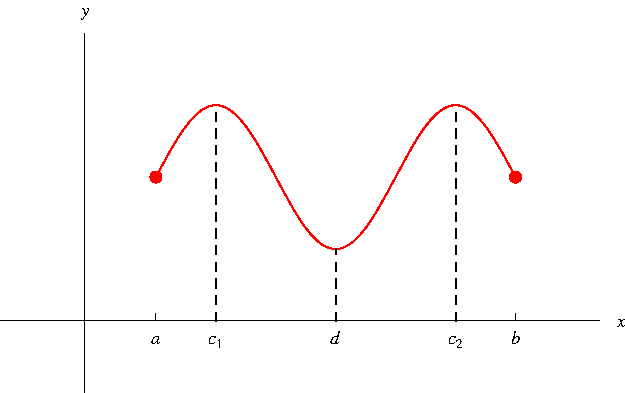
\includegraphics[width=4cm]{maxima-minima/pictures/04-01-evtc.pdf}%
}%
\end{columns}
\begin{itemize}
\item<2-| alert@2>  Extreme values might happen at endpoints.
\item<3-| alert@3>  Extreme values might happen twice.
\end{itemize}
\end{frame}
% end module EVT-statement

%\begin{frame}
\begin{example}
A cone is folded from a wedge-shaped profile of radius $r$. Find the maximal possible volume $V$ of such a cone.

\begin{columns}[c]
\column{.27\textwidth}
%Please note: the below pictures are up to scale. The cone is an isogonal projection onto the tangent plane to the sphere centered at the origin and passing through point (0, 2, 0.4). The function used to draw the cone is 
%the vector partition calculator function plotConeUsualProjection(3/4, \sqrt(1-DoubleValue{}(3/4)^2), 2, 0.4)
\psset{xunit=1.5cm, yunit=1.5cm}
\begin{pspicture}(-5, -5)(5,5) 
\psframe*[linecolor=white](-5,-5)(5,5) 
\tiny 
\pscustom*[linecolor=cyan!30]{ \psparametricplot[algebraic] {2.35619}{7.06858} {0+1*cos(t)| 0+1*sin(t)} \psline(0.707107, 0.707107)(0, 0)(-0.707107, 0.707107)}

\psparametricplot[algebraic,linecolor=blue]{2.35619}{7.06858}{cos(t)| sin(t)} 
\psline[linecolor=red](0.707107, 0.707107)(0, 0)(-0.707107, 0.707107)

\rput[t](0.35, 0.30){$r$}
\rput[lb](0.8,0.8){$B$}
\rput[rb](-0.8,0.8){$A$}
\rput[b](0,0.1){$O$}

\uncover<7->{
\psparametricplot[algebraic,linecolor=purple]{2.35619}{7.06858}{0.07*cos(t)| 0.07*sin(t)} 
\rput[t](0, -0.1){$\alert<7>{\theta}$}
}
\uncover<8->{
\psparametricplot[linewidth=1pt, algebraic,arrows=<->, linecolor =blue] {4.41238898} {5.01238898}{cos(t)| sin(t)} 
}
\uncover<9->{
\rput[b](0, -0.9){\alert<9>{$r\theta$}}
}
\psline[linecolor=red!1](-1.03,-1.03)(-1.03,-1.02)
\end{pspicture} 

\psset{xunit=1.5cm, yunit=1.5cm}
\begin{pspicture}(-5, -5)(5,5) 
\psframe*[linecolor=white](-5,-5)(5,5) 
\tiny 
\rput[b](0,0.7){$O$}
\rput[l](0.8, 0.0333562){$A$}

\psline[linecolor=\psColorGraph](0.73046, 0.0333562)(0, 0.648593)
\psline[linecolor=\psColorGraph](-0.73046, 0.0333562)(0, 0.648593)
\psparametricplot[algebraic,linecolor=blue]{-3.37036}{0.228769}{0.75*cos(t) |0.147087*sin(t)}
\psparametricplot[algebraic, linestyle=dashed, linecolor=blue] {0.228769}{2.91282}{0.75*cos(t) |0.147087*sin(t)}
\rput[bl](0.38,0.34 ){$r$}

\uncover<10,11>{
\psparametricplot[algebraic,linecolor=red]{-3.37036}{0.228769}{0.75*cos(t) |0.147087*sin(t)}
\psparametricplot[algebraic, linestyle=dashed, linecolor=red] {0.228769}{2.91282}{0.75*cos(t) |0.147087*sin(t)}
\rput[bl](0.38,0.34 ){$r$}
}

\psline[linecolor=red!1](-1, 0)(-0.99,0)
\psline[linecolor=red!1](0.99, 0)(1,0)
\uncover<2->{
\psline[linecolor=black](0,0)(0,0.648593)
\rput[r](-0.07,0.32){$h$}
}
\uncover<3->{
\psline[linecolor=black](0,0)(0.73046, 0.0333562)
\psline[linecolor=black](0.073046, 0.00333562) (0.073046, 0.0764577) (0, 0.0731221)
\rput[t](0.35, -0.02){$t$}
}
\end{pspicture} 

\psset{xunit=1.5cm, yunit=1.5cm}
\begin{pspicture}(-5, -5)(5,5) 
\psframe*[linecolor=white](-5,-5)(5,5) 
\tiny 
\uncover<13->{
\rput[b](0,0.7){$O$}
\rput[l](0.8, 0){$A$}
\rput[r](-0.05,0.32){\alert<13,14>{$h$}}
\rput[t](0.38,-0.05){$\alert<14>{t}$}
\rput[bl](0.38,0.34 ){$\alert<14>{r}$}
\psline(0,0)(0.75,0)
\psline[linecolor=\psColorGraph](0.75,0)(0, 0.648593)
\psline(0, 0.648593)(0,0)
\psline(0.075, 0)(0.075, 0.075)(0, 0.075)
}
\psline[linecolor=red!1](-1, -0.147087)(-0.99,-0.147087)
\psline[linecolor=red!1](0.99, 0.8)(1,0.8)
\end{pspicture} 

\vspace{0.9cm}
\column{.73\textwidth}
\only<1-20>{
\uncover<2->{
Set $h$ - cone height,} \uncover<3->{$t$ - cone radius.} \uncover<4->{Then $\alert<4,17>{V=} \uncover<5->{\alert<5>{\frac{1}3 (\alert<6>{\text{area cone base}})h} }\uncover<6->{=\alert<17>{ \frac13 \alert<6>{\pi   t^2} h }}$.} \uncover<7->{ Let $\alert<7>{\theta}$ - angle of the wedge.} \uncover<8->{Then $ \alert<8,9>{\text{arc}{AB}=} \uncover<9->{\alert<9,12>{r\theta}}$ \uncover<10->{\alert<10,11>{= perimeter cone base =}} $\uncover<11->{\alert<11,12>{2\pi t}.}$} \uncover<12->{Therefore $\alert<12,15,18>{t=\frac{r\theta}{2\pi}}$.} \uncover<13->{Then 

$\displaystyle
\alert<13,14,19>{h=}  \uncover<14->{ \alert<14>{ \sqrt{ r^2- \alert<15>{t}^2 }}} \uncover<15->{= \sqrt{r^2- \left(\alert<15>{ \frac{r\theta}{ 2\pi}}\right)^2}}\uncover<16->{=\alert<19>{\frac{r}{2\pi }\sqrt{ 4\pi^2-\theta^2 }},}
$
}%13 

\uncover<17->{
and therefore 

$
\begin{array}{rcl}
\alert<17>{V}&\alert<17>{=}&\displaystyle\alert<17>{ \frac13\pi \alert<18>{t}^2 \alert<19>{h}}= \uncover<18->{\frac13\pi \left(\alert<18>{\frac{r\theta}{2\pi}}\right)^2\alert<19>{\frac{r}{2\pi}\sqrt{4\pi^2-\theta^2}}}\\ 
\uncover<20->{&=& \displaystyle \frac{r^3}{24\pi^2} \theta^2\sqrt{4\pi^2-\theta^2}\quad . }
\end{array}
$
}
}
\only<21-24>{
\noindent We reduced the problem to: find the maximum of

$
V=\displaystyle \frac{r^3}{24\pi^2} \theta^2\sqrt{4\pi^2-\theta^2},\quad \quad  \uncover<22->{\alert<22,23>{\uncover<23->{0} \leq \theta \leq \uncover<23->{2\pi}}} 
$

as function of $\theta$ (using the \alert<22, 23>{closed interval} method).

\uncover<24->{We need to find the critical points of $V$, i.e., the values of $\theta$ for which $\frac{dV}{d\theta}=0$ and the values of $\theta$ for which  $\frac{dV}{d\theta}$ is not defined.}
}
\only<25-35>{
\noindent $
\begin{array}{rcl}
V&=&\displaystyle \frac{r^3}{24\pi^2} \theta^2\sqrt{4\pi^2-\theta^2}, \quad \quad \quad 0\leq \theta \leq2\pi \\
\displaystyle \uncover<26->{\displaystyle\frac{dV}{d\theta} &=&} \displaystyle \uncover<27->{\phantom{+}\left(\frac{r^3}{24\pi^2}\right)   \alert<28,29>{\frac{d}{d\theta}\left(\theta^2\right)} \sqrt{4\pi^2-\theta^2}}\\
&&\uncover<27->{\displaystyle+\left(\frac{r^3}{24\pi^2}\right)\theta^2\alert<30,31>{\frac{d}{ d\theta}\left(\sqrt{4\pi^2-\theta^2} \right)}} \\
\uncover<28->{&=& \displaystyle \phantom{+}\left(\frac{r^3}{24\pi^2}\right) \alert<28,29>{( \uncover<29->{\alert<29,33>{2\theta}})} \alert<33>{\sqrt{4\pi^2-\theta^2}}}\\
&&\displaystyle\uncover<28->{ +\left(\frac{r^3}{24\pi^2}\right) \alert<34>{\theta^2} \alert<30,31,34>{\left(\uncover<31->{ \frac{1}{2} \frac{ \frac{d}{d\theta} (-\theta^2)}{\sqrt{4\pi^2-\theta^2}}}\right)}  } \\
\uncover<32->{&=&\displaystyle\left(\frac{r^3}{24\pi^2}\right)\frac{ \alert<33>{2\theta(4\pi^2-\theta^2)}\alert<34>{-\theta^3} }{\alert<33,34>{ \sqrt{4\pi^2-\theta^2}}}}\\
\uncover<35->{&=&\displaystyle\left(\frac{r^3}{24\pi^2}\right)\frac{8 \theta \pi^2-3\theta^3 }{\sqrt{4\pi^2-\theta^2}}}
\end{array}
$
}
\only<36-44>{
$
\begin{array}{rcl}
V&=&\displaystyle \frac{r^3}{24\pi^2} \theta^2\sqrt{4\pi^2-\theta^2}, \quad \quad \quad \alert<43>{0\leq \theta \leq2\pi} \\
\displaystyle \frac{dV}{d\theta}&=& \displaystyle\left(\frac{r^3 } {24\pi^2} \right)\frac{\alert<38>{8\theta\pi^2-3\theta^3} }{\sqrt{4\pi^2-\theta^2}}
\end{array}
$

\uncover<37->{We have that $\frac{dV}{d\theta}=0$ when }
$
\begin{array}{rcl}
\uncover<38->{ \alert<38>{8\theta\pi^2-3\theta^3}&=&0}\\
\uncover<39->{\theta(8\pi^2-3\theta^2)&=&0}\\
\uncover<40->{-3\alert<41>{\theta}\alert<42>{\left(\theta-\sqrt{\frac{8}{3}}\pi \right)} \alert<43>{\left(\theta+\sqrt{\frac{8}{3}}\pi \right)}&=&0.}
\end{array}
$

\uncover<41->{Therefore $\theta$ is critical point for $V$ if $\alert<41>{\theta= 0}$ or $\alert<42>{\theta=\sqrt{\frac83}\pi }$,} \uncover<43->{(note $\alert<43>{\theta=-\sqrt{\frac83}\pi}$ is outside of the domain of $V$).} \uncover<44->{For $\theta=0,2\pi$ the volume $V$ is $0$, so the maximum 
volume is attained at $\theta=\sqrt{\frac83}\pi$.}
} %frame36
\only<45->{
\[
V(\alert<46>{\theta} )=\displaystyle \frac{r^3}{24\pi^2} \alert<46>{\theta}^2 \sqrt{4 \pi^2 - \alert<46>{\theta}^2} 
\]
Finally, the answer to the problem is
$
\begin{array}{rcl}
V_{max}&=&\displaystyle V\left(\alert<46>{ \sqrt{\frac83} \pi} \right)\\
\uncover<46->{ &=&\displaystyle \frac{r^3}{\alert<47>{24}\alert<48>{\pi^2}} \left( \alert<46>{ \alert<47>{\sqrt{\frac83}} \alert<48>{\pi}} \right)^{\alert<47,48>{2}} \sqrt{4 \alert<48>{\pi^2} -\left( \alert<46>{ \sqrt{\frac83} \alert<48>{\pi}} \right)^{\alert<48>{2}}}}\\
\uncover<47->{ &=&\displaystyle \frac{r^3}{\alert<47>{9}} \alert<48>{\pi} \sqrt{\alert<49>{4-\frac{8}3}}}\\
\uncover<49->{&=& \displaystyle \pi\frac{r^3}9 \sqrt{ \alert<49>{\frac43}}} \uncover<50>{=\frac{2\pi r^3}{9\sqrt3}}
\end{array}
$
}

\end{columns}
\uncover<3>{}
\end{example}
\end{frame} 
%\begin{frame}
\frametitle{Pascal triangle motivation}
\begin{problem}
Find a general formula for the expansion of $(a+b)^n$.
\end{problem}
\tiny
\begin{tabular}{ccccccccccccc}
$a+b$     &$=$&&&&& $\alert<6>{a}$ &$+$& $\alert<6>{b}$ \\
$(a+b)^2$ &$=$&&&& $\alert<7>{a^2}$ &$+$& $\alert<6,7>{\alert<3>{2}ab}$&$+$&$b^2$ \\
$(a+b)^3$ &$=$&&& $a^3$ &$+$& $\alert<7,8>{\alert<3>{3}a^2b}$& $+$& $\alert<8>{\alert<3>{3}ab^2}$& $+$&$b^3$ \\
$(a+b)^4$ &$=$& &$a^4$&$+$&$\alert<9>{\alert<3>{4}a^3b}$ &$+$& $\alert<8,9>{\alert<3>{6}a^2b^2}$&$+$& $\alert<3>{4}ab^3$&$+$&$b^4$ \\
$(a+b)^5$ &$=$& $a^5$ &$+$& $\alert<3>{5}a^4b$& $+$& $\alert<9>{\alert<3>{10}a^3b^2}$ &$+$&$\alert<3>{10}a^2b^3 $&$+$&$\alert<3>{5}ab^4$&$+$&$b^5$ \\
&&\multicolumn{11}{c}{$\vdots$}
\\ \hline \hline
\uncover<2->{\uncover<14>{row 0}&&&&&&&$\alert<11>{1}$}\\
\uncover<2->{\uncover<14>{row 1}&&&&&& $\alert<6,11>{1}$&&$\alert<6,11,14>{1}$}\\
\uncover<2->{\uncover<14>{row 2} &&&&&$\alert<7,11>{1}$&&$\alert<3,6,7,12,14>{2}$&&$\alert<11>{1}$}\\
\uncover<2->{\uncover<14>{row 3} &&&& $\alert<11>{1}$&&$\alert<3,7,8,12,14>{3}$&&$\alert<3,8,12>{3}$&&$\alert<11>{1}$}\\
\uncover<2->{\uncover<14>{row 4}&&&$\alert<11>{1}$&&$\alert<3,9,12,14>{4}$&&$\alert<3,8,9,13>{6}$&&$\alert<3,12>{4}$&&$\alert<11>{1}$}\\
\uncover<2->{\uncover<14>{row 5} &&$\alert<11>{1}$&&$\alert<3,12,14>{5}$&&$\alert<3,9,13>{10}$&&$\alert<3,13>{10}$&&$\alert<3,12>{5}$&&$\alert<11>{1}$}\\
\uncover<2->{&&\multicolumn{11}{c}{$\vdots$}}\\
\end{tabular}
\normalsize
\begin{itemize}
\item \uncover<2->{\alert<3>{Arrange the coefficients of the formulas in a triangle.}}
\item \uncover<4->{{The triangle is named after Blaise Pascal(1623-1662).}}
\item \uncover<5->{{\alert<5->{Observe:} each entry $=$ sum two entries above. }} \only<6>{\alert<6>{$1+1=2$}}\only<7>{\alert<7>{$1+2=3$}} \only<8>{\alert<8>{$3+3=6$}}\only<9>{\alert<9>{$4+6=10$}} \only<10>{and so on...}
\item \uncover<11->{\alert<11-13>{Triangle is symmetric. }} \uncover<14->{\alert<14>{Second entry in row is the row number. } }
\end{itemize}


\end{frame}
\begin{frame}
\frametitle{Pascal triangle definition}
\begin{itemize}
\item<1->Previous slide: the coefficients in the expansion of $(a+b)^n$ can be arranged in triangular fashion. This slide we pretend to forget that.
\item<1-> Define a triangular arrangement of numbers:
\item<2-> write $1$'s on two sides of triangle arranged as shown below; 
\item<3-> define the remaining entries by requesting each number is the sum of the two entries above it. 
\end{itemize}
\begin{definition} 
\uncover<4->{ The so defined triangle is called Pascal's triangle. }
\end{definition}
\tiny
\begin{tabular}{ccccccccccccc}
&&&&&&&$\uncover<2->{\alert<2,4>{1}}$\\
&&&&&& $\uncover<2->{\alert<2,4>{1}}$&&$\uncover<2->{\alert<2,4>{1}}$\\
&&&&& $\uncover<2->{\alert<2,4>{1}}$ &&$\uncover<3->{ \alert<4>{2}}$ &&$\uncover<2->{\alert<2,4>{1}}$\\
&&&& $\uncover<2->{\alert<2,4>{1}}$&& $\uncover<3->{\alert<4>{3}}$ &&$\uncover<3->{\alert<4>{3}}$&&$\uncover<2->{\alert<2,4>{1}}$\\
&&& $\uncover<2->{\alert<2,4>{1}}$&&$\uncover<3->{\alert<4>{4}}$&&$\uncover<3->{\alert<4>{6}}$&&$\uncover<3->{\alert<4>{4}}$&& $\uncover<2->{\alert<2,4>{1}}$\\
&&$\uncover<2->{\alert<2,4>{1}}$&&$\uncover<3->{\alert<4>{5}}$&&$\uncover<3->{ \alert<4>{10}}$&&$\uncover<3->{\alert<4>{10}}$&&$\uncover<3->{\alert<4>{5}}$&&$\uncover<2->{\alert<2,4>{1}}$\\
&&\multicolumn{11}{c}{$\vdots$}\\
\end{tabular}
\normalsize


\end{frame}
%% begin module concavity-def
\begin{frame}
\frametitle{What Does $f''$ Say About $f$?}
$f$ and $g$ are both increasing on $(a,b)$, but ``bend'' in different directions.
\begin{columns}[c]
\column{.5\textwidth}
\psset{xunit=0.6cm, yunit=0.6cm}
\begin{pspicture}(-1,-1)(4,3.8)
\psframe*[linecolor=white](-1,-1)(4,3.8)
\psaxes[ticks=none, labels=none]{<->}(0,0)(-1,-1)(4,3.8)
%Function formula: 1/2+1/4 ((-1+x)^{2})+1/4 (x) =1/4x^{2}-1/4x +3/4
\psplot[linecolor=red, plotpoints=1000]{-1}{4}{x 0.25 mul x -1 add 2 exp 0.25 mul add 0.5 add }
\tiny
\rput(1, 2){$y=f(x)$}
\psXTickWithLabel{0.5}{$a$} 
\psXTickWithLabel{3.7}{$b$} 

\uncover<3>{ %point: x=0.3
%Function formula: -1/10 (x)+291/400 
\psplot[linecolor=blue, plotpoints=1000]{-0.5}{4}{0.7275 x -0.1 mul add }
}
\uncover<4->{%point: x=0.3
%Function formula: -1/10 (x)+291/400 
\psplot[linecolor=blue, plotpoints=1000]{0}{0.6}{0.7275 x -0.1 mul add } 
}
\uncover<3->{
\psFullDot{0.3}{0.6975}
}

\uncover<4>{ %point x=1.3
%Function formula: 2/5 (x)+131/400 
\psplot[linecolor=blue, plotpoints=1000]{-0.5}{4}{0.3275 x 0.4 mul add } 
}
\uncover<5->{ %point x=1.3
%Function formula: 2/5 (x)+131/400 
\psplot[linecolor=blue, plotpoints=1000]{1}{1.6}{0.3275 x 0.4 mul add } 
}
\uncover<4->{
\psFullDot{1.3}{0.8475}
}

\uncover<5>{ %point x=2.3
%Function formula: 9/10 (x)-229/400 
\psplot[linecolor=blue, plotpoints=1000]{0.080555556}{4}{-0.5725 x 0.9 mul add } 
}
\uncover<6->{ %point x=2.3
%Function formula: 9/10 (x)-229/400 
\psplot[linecolor=blue, plotpoints=1000]{2}{2.6}{-0.5725 x 0.9 mul add } 
}
\uncover<5->{
\psFullDot{2.3}{1.4975}
}

\uncover<6>{ %point x=3.3
%Function formula: 7/5 (x)-789/400 
\psplot[linecolor=blue, plotpoints=1000]{1.051785714}{4}{-1.9725 x 1.4 mul add } 
}
\uncover<7->{  %point x=3.3
%Function formula: 7/5 (x)-789/400 
\psplot[linecolor=blue, plotpoints=1000]{3}{3.6}{-1.9725 x 1.4 mul add } 
}
\uncover<6->{
\psFullDot{3.3}{2.6475}
}
\uncover<9>{
\psline[linecolor=blue](-1, 1.25) (1.6, 0.99)
}
\uncover<10->{
\psline[linecolor=blue!30](-1, 1.25) (1.6, 0.99)
}
\uncover<10>{
\psline[linecolor=blue](0, 0.75) (2.6, 1.79)
}
\uncover<11->{
\psline[linecolor=blue!30](0, 0.75) (2.6, 1.79)
}
\uncover<11>{
\psline[linecolor=blue](1, 0.75) (3.6, 3.09)
}
\uncover<12->{
\psline[linecolor=blue!30](1, 0.75) (3.6, 3.09)
}

\rput[t](2,-0.5) {\uncover<6->{Concave up}}
\end{pspicture} 
%\ \only<handout:0| -2>{%
%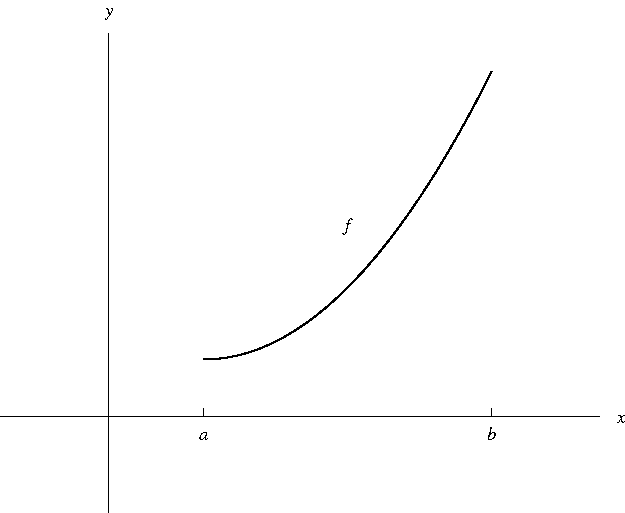
\includegraphics[height=3.5cm]{curve-sketching/pictures/04-03-concaveupa.pdf}%
%}%
%\only<handout:0| 3>{%
%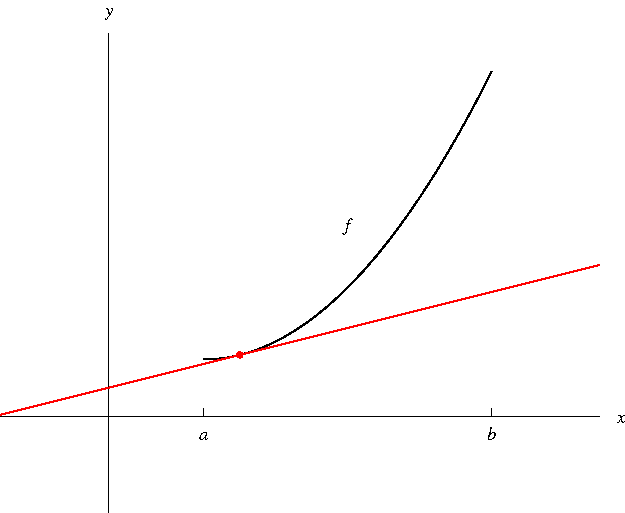
\includegraphics[height=3.5cm]{curve-sketching/pictures/04-03-concaveupb.pdf}%
%}%
%\only<handout:0| 4>{%
%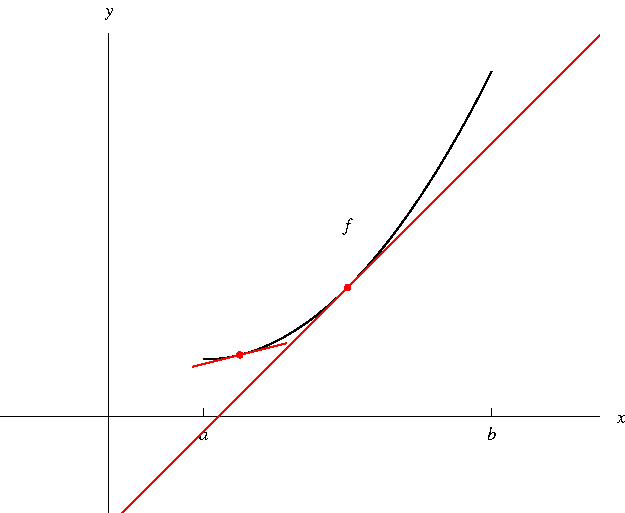
\includegraphics[height=3.5cm]{curve-sketching/pictures/04-03-concaveupc.pdf}%
%}%
%\only<handout:0| 5>{%
%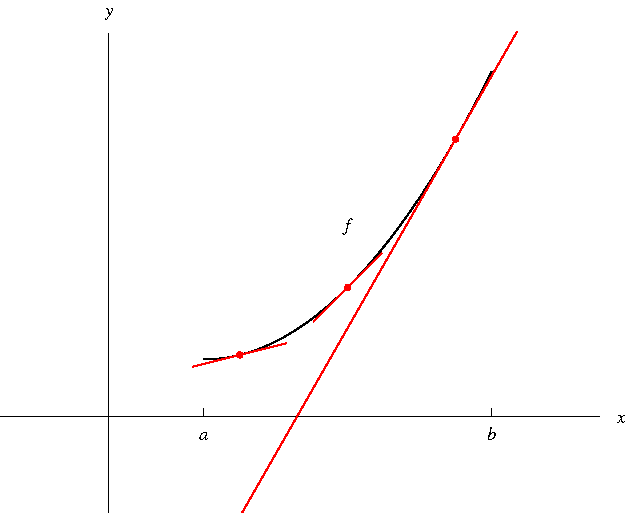
\includegraphics[height=3.5cm]{curve-sketching/pictures/04-03-concaveupd.pdf}%
%}%
%\only<6->{%
%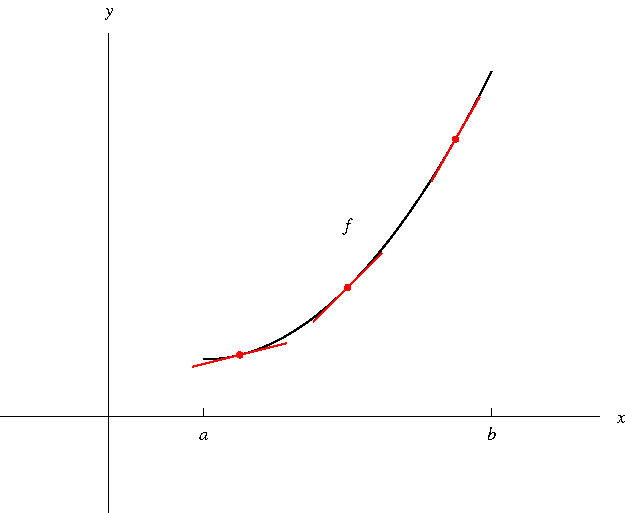
\includegraphics[height=3.5cm]{curve-sketching/pictures/04-03-concaveupe.pdf}%
%}%


\column{.5\textwidth}
\psset{xunit=0.6cm, yunit=0.6cm}
\begin{pspicture}(-1,-1)(4,3.8)
\psframe*[linecolor=white](-1,-1)(4,3.8)
\psaxes[ticks=none, labels=none]{<->}(0,0)(-1,-1)(4,3.8)
\tiny
\rput[l](2.5, 0.7){$y=g(x)$}
%Function formula: -1/4x^{2}+5/4x +1/2=11/4-1/4 (-3+x)^{2}-1/4 x 
\psplot[linecolor=red, plotpoints=1000]{-1}{4}{x -0.25 mul x -3 add 2 exp -0.25 mul add 2.75 add }
\psXTickWithLabel{0.3}{$a$} 
\psXTickWithLabel{2.5}{$b$} 


\uncover<3>{
%Function formula: 11/10 (x)+209/400 
\psplot[linecolor=blue, plotpoints=1000]{-0.5}{2.979}{0.5225 x 1.1 mul add }
}
\uncover<4->{ 
%Function formula: 11/10 (x)+209/400 
\psplot[linecolor=blue, plotpoints=1000]{0}{0.6}{0.5225 x 1.1 mul add } 
}
\uncover<3->{
\psFullDot{0.3}{0.8525}
}
\uncover<4>{
%Function formula: 3/5 (x)+369/400 
\psplot[linecolor=blue, plotpoints=1000]{-0.5}{4}{0.9225 x 0.6 mul add } 
}
\uncover<5->{
%Function formula: 3/5 (x)+369/400 
\psplot[linecolor=blue, plotpoints=1000]{1}{1.6}{0.9225 x 0.6 mul add } 
}
\uncover<4->{
\psFullDot{1.3}{1.7025}
}

\uncover<5>{
%Function formula: 1/10 (x)+729/400 
\psplot[linecolor=blue, plotpoints=1000]{-0.5}{4}{1.8225 x 0.1 mul add } 
}
\uncover<6->{
%Function formula: 1/10 (x)+729/400 
\psplot[linecolor=blue, plotpoints=1000]{2}{2.6}{1.8225 x 0.1 mul add } 
}
\uncover<5->{
\psFullDot{2.3}{2.0525}
}
\uncover<6>{
%Function formula: -2/5 (x)+1289/400 
\psplot[linecolor=blue, plotpoints=1000]{-0.5}{4}{3.2225 x -0.4 mul add } 
}
\uncover<7->{
%Function formula: -2/5 (x)+1289/400 
\psplot[linecolor=blue, plotpoints=1000]{3}{3.6}{3.2225 x -0.4 mul add } 
}
\uncover<6->{
\psFullDot{3.3}{1.9025}
}
\rput[t](2,-0.5) {\uncover<6->{Concave down}}
\uncover<9>{
\psline[linecolor=blue] (-1, -1) (1.6, 1.86)
}
\uncover<10->{
\psline[linecolor=blue!30] (-1, -1) (1.6, 1.86)
}
\uncover<10>{
\psline[linecolor=blue] (0, 0.5) (2.6, 2.06)
}
\uncover<11->{
\psline[linecolor=blue!30] (0, 0.5) (2.6, 2.06)
}
\uncover<11>{
\psline[linecolor=blue] (1, 1.5) (3.6, 1.76)
}
\uncover<12->{
\psline[linecolor=blue!30] (1, 1.5) (3.6, 1.76)
}

\end{pspicture} 
%\ \only<handout:0| -2>{%
%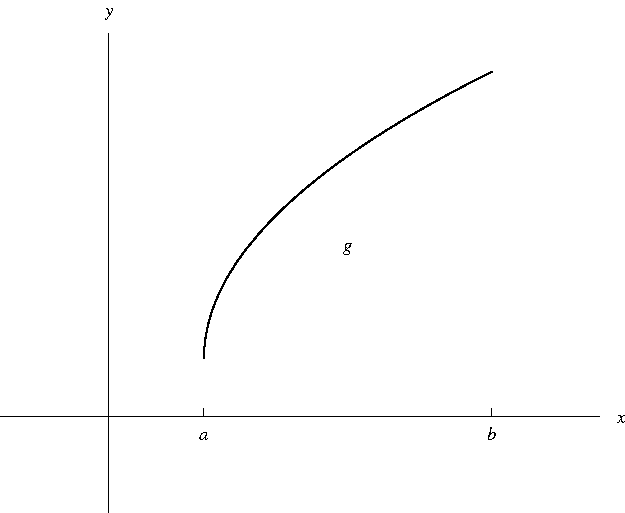
\includegraphics[height=3.5cm]{curve-sketching/pictures/04-03-concavedowna.pdf}%
%}%
%\only<handout:0| 3>{%
%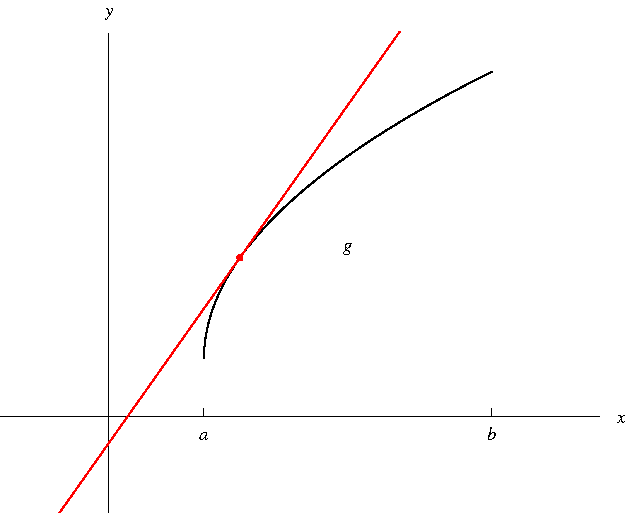
\includegraphics[height=3.5cm]{curve-sketching/pictures/04-03-concavedownb.pdf}%
%}%
%\only<handout:0| 4>{%
%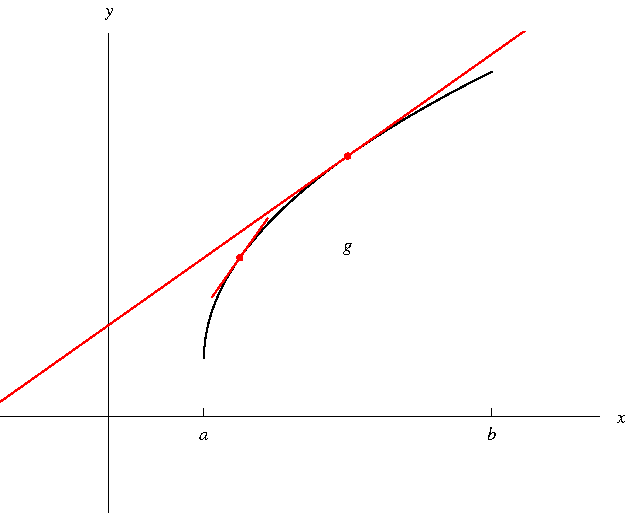
\includegraphics[height=3.5cm]{curve-sketching/pictures/04-03-concavedownc.pdf}%
%}%
%\only<handout:0| 5>{%
%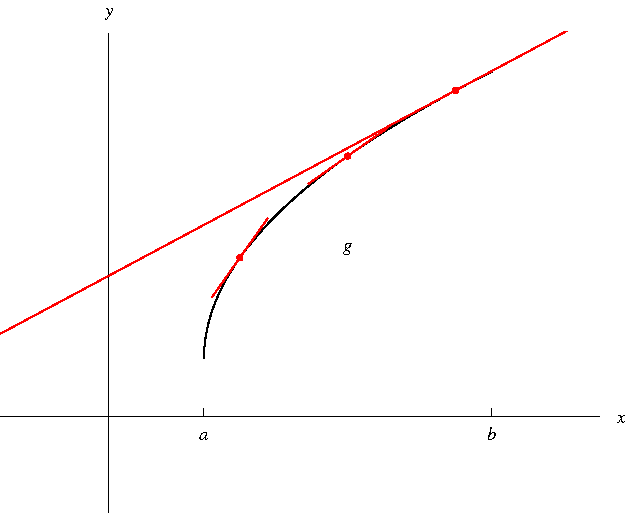
\includegraphics[height=3.5cm]{curve-sketching/pictures/04-03-concavedownd.pdf}%
%}%
%\only<6->{%
%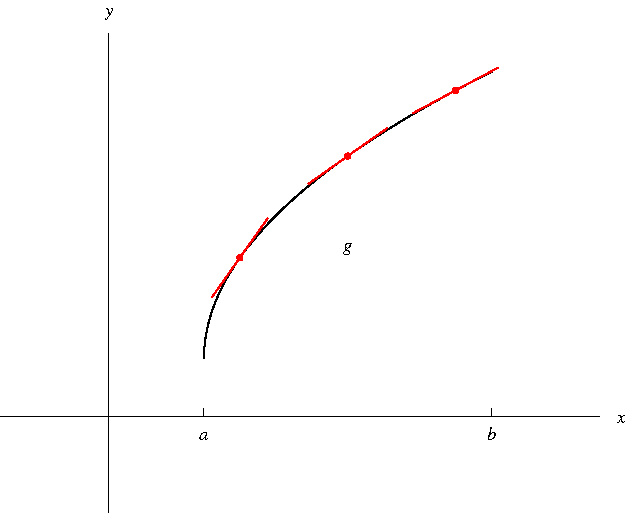
\includegraphics[height=3.5cm]{curve-sketching/pictures/04-03-concavedowne.pdf}%
%}%
\end{columns}
\uncover<8-12>{%
\begin{definition}[Concave Up/Concave Down, most general definition]
A function is called concave up/down if the line segment between any two points on its graph lies above/below the graph.
\end{definition}
}%
\uncover<2->{
\begin{theorem}[Can be taken as a definition]
Let $f$ be a differentiable function on an interval $I$. Then $f$ is
concave up (on $I$) if its graph lies above all of its tangents (on $I$), and $f$ is concave down (on $I$) if its graph lies below all of its tangents (on $I$).
\end{theorem}
}
\end{frame}
% end module concavity-def

%% begin module inflection-point-def
\begin{frame}
\begin{definition}[Inflection Point]
A point $P$ on a curve $y = f(x)$ is called an inflection point if $f$ is continuous at $P$ and the curve changes from concave up to concave down or from concave down to concave up at $P$.
\end{definition}
\uncover<2->{%
Another way of saying this is that $P$ is an inflection point if $f''$ changes signs at $P$.
}%
\end{frame}
% end module inflection-point-def

% end lecture
%% begin module differential-def
\begin{frame}
\frametitle{Differentials}
\begin{itemize}
\item<1-> From previous slides:
\alert<12>{$\displaystyle \Delta y\approx \frac{dy}{dx} \Delta x$}
\item $\displaystyle \only<1-2>{\Delta y} 
\only<3->{\alert<3,6> {\alert<7>{d}y}} \only<1-3>{\approx}
\only<4->{\alert<3> =} \only<1->{\frac{dy}{\alert<5>{dx}}}
\only<1-3>{ \Delta x} 
\only<4->{\alert<4,5,8>{\alert<7>{d}x}}
\only<6->{=\alert<6>{\alert<7>{d}y} }
$
\item<2-> If we substitute \alert<3>{$\Delta y $ by the formal expression $dy$} and \alert<4>{$\Delta x$ by the formal expression $dx$}, the expression \alert<5>{$dx$ appears to ``cancel''} to give a \alert<6>{formal identity}.
\item<7-> Define the \alert<7,11>{\emph{differential $d$}} %\uncover<8->
{ and the \alert<8,10>{\emph{differential forms $dx$, $d(f(x))$}}} %\uncover<9->
{by requesting that \alert<9>{$d$ and $dx$ satisfy the transformation law} 
\[
\alert<9>{\alert<8>{\alert<7>{d}(f(x))}=f'(x) \alert<8>{\alert<7>{d}x}}
\] 
for any differentiable function $f(x)$.} In abbreviated notation:
\[ 
\alert<9>{ \alert<7>{d}f = f' \alert<8>{\alert<7>{d}x}}
\]
\uncover<10->{Expressions containing expression of the form $\alert<10>{\alert<11>{d}(something)}$ are called \alert<10>{differential forms}.}
\item<12-> Differential forms ``encode'' linear approximations.
\end{itemize}
\end{frame}
\begin{frame}
\begin{itemize}
\item $\alert<4,8,11>{\alert<3>{ \alert<2>{d} f(x)}= f' \alert<3>{\alert<2>{d}x}}$.
\item<2-> On the previous slide we stated the \alert<2>{differential $d$} and the \alert<3>{differential forms} $\alert<3>{dx, d f(x)}$ are \alert<4,7>{formal expressions related by a transformation law}.
\item<5-> One can construct differential forms and differentials  directly but this is outside of the scope of Calculus I and II. 
\item<6-> Courses such as ``Integration and Manifolds'' or ``Differential geometry'' usually give the precise definitions.
\item<7-> Nonetheless, \alert<7>{what we studied} is \alert<8>{completely sufficient} for practical purposes and \alert<8>{carrying out computations}.
\item<9-> \alert<9,10>{\textbf{Do not confuse differentials with derivatives.}} \uncover<11->{\alert<11>{The correct equality is this.}}

\[
\only<9>{\alert<9,10>{ df(x) = f'(x)}} \only<10->{\alert<9,10>{ \xcancel{df(x) = f'(x)}}}
\quad \quad \quad\quad \quad\uncover<11>{\alert<11>{ df(x)=f'(x)dx}}
\]
\end{itemize}
\end{frame}

%\begin{frame}
\begin{example}
Compute the differential (via $\diff x$).

\[
\alertNoH{2}{\diff\left(x^2\right)}\uncover<2->{\alertNoH{2}{= \alertNoH{3}{\left(x^2\right)'} \diff x} } \uncover<3->{=\alertNoH{3}{2x} \diff x\quad .}
\]
\end{example}
\end{frame}
\begin{frame}
\begin{example}
Compute the differential (via $\diff x$).
\[
\alertNoH{2}{\diff \left(\sqrt{x}\right)} \uncover<2->{= \alertNoH{2}{\alertNoH{3}{\left(\sqrt{x}\right)'}\diff  x} \uncover<3>{= \alertNoH{3}{ \frac{1}{2\sqrt{x}}} \diff x \quad .}}
\]
\end{example}
\end{frame}


%%begin module differentials-rules
\begin{frame}
\begin{itemize}
\item All rules for computing with derivatives have analogues for computing with differential forms.
\item<2-> The rules for computing differential forms are a direct consequence of the corresponding derivative rules and the transformation law $\diff (f(x))=f'(x)\diff x$.
\end{itemize}
\end{frame}
\begin{frame}
Rule name: \phantom{p}
\only<1,2>{\alertNoH{1,2}{product rule. }}
\only<3,4>{\alertNoH{3,4}{constant derivative rule. }}
\only<7,8>{\alertNoH{7,8}{sum rule. }}
\only<9,10>{\alertNoH{9,10}{chain rule. }}
\only<11-12>{\alertNoH{11-12}{power rule. }}
\only<13-14>{\alertNoH{13-14}{exponent derivative rule. }}
%\only<5,6>{\alertNoH{5,6}{ Constant derivative rule. }}

\begin{tabular}{lll}
Differential rule & Derivative rule\\
\uncover<2->{$\diff (fg)=g \diff f +f \diff g$} &
\uncover<1->{$(fg)'=f'g +f g'$} \\
\uncover<4->{$\diff c=0 {\color{gray!50}{ =0\diff x}}$} &
\uncover<3->{$(c)'=0$ & $c$-const.}\\
\uncover<6->{$\diff (cf)=c\diff f $} &
\uncover<5->{$(cf)'=cf'$ &$c$-const. }\\
\uncover<8->{$\diff (f+g)=\diff f +\diff g$} &
\uncover<7->{$(f+g)'=f'+g'$}\\
\uncover<10->{$\diff f(g(x))=$ $ f'(g(x))\diff g(x) $}\\
\uncover<10->{$\phantom{\diff f(g(x))}=$ $ f'(g(x))g'(x)\diff x$} &
\uncover<9->{$(f(g(x)))'= f'(g(x))g'(x)$} \\
\uncover<10->{$\diff f(g)\phantom{(x)}=f'(g)\diff g$} \\\hline
\uncover<12->{$\diff \left( x^n\right)= nx^{n-1}\diff x$} &
\uncover<11->{$(x^n)'=nx^{n-1}$}\\
\uncover<14->{$\diff  \left(e^x\right)= e^x \diff x$} &
\uncover<13->{$\left(e^x\right)'=e^x$}\\
\uncover<16->{$\diff \left(\sin x\right) = \cos x \diff x$} &
\uncover<15->{$(\sin x)'= \cos x$}\\
\uncover<18->{$\diff \left(\cos x \right)= -\sin x \diff x$} &
\uncover<17->{$(\cos x)'= -\sin x$}\\
\uncover<20->{$\displaystyle \left(\diff \ln x\right) =\frac{1}{x}\diff x$} &
\uncover<19->{$\left(\ln x\right)' =\displaystyle \frac1x$}\\
\end{tabular}


\end{frame}
%end module differentials-rules

\begin{frame}
Differentials are especially efficient at ``encoding'' the chain rule.
\begin{example}
Compute the differential $\diff  \ln \left(1+\sqrt{1+x^2}\right)$.

\uncover<3->{Set $\alertNoH{3,6,15}{u=1+\sqrt{1+x^2}}$.} \uncover<8->{Set $\alertNoH{8,11,16}{v=1+x^2}$. }

\[
\begin{array}{rcl}
\displaystyle\uncover<2->{\diff \ln \left(\alertNoH{3}{1 +\sqrt{1 +x^2}}\right) &=&}\displaystyle \uncover<3->{ \alertNoH{4,5}{\diff \ln \alertNoH{3}{ u}=}} \uncover<5->{\alertNoH{5}{\frac{1}{u}\diff  \alertNoH{6}{u}}=}\uncover<6->{\frac{1}{u}\diff \left(\alertNoH{6}{1+\sqrt{ 1+x^2}}\right) =}\\
&\uncover<7->{=}&\uncover<7->{\displaystyle\frac{1}u \diff \sqrt{\alertNoH{8}{1+x^2}}=} \uncover<8->{\frac{1}u \alertNoH{9}{ \diff  \alertNoH{8}{v}^{\frac12}}=} \uncover<9->{ \frac1 u \alertNoH{9}{\frac{1}{2} \alertNoH{10}{v^{-\frac12}} \diff  \alertNoH{11}{v}} }\\
&\uncover<10->{=} &\displaystyle \uncover<10->{ \frac{\alertNoH{10}{1} } {2u\alertNoH{10}{v^{\frac12}}} \alertNoH{12}{\diff  ( \alertNoH{11}{1+x^2})}=} \uncover<12->{\frac{\alertNoH{12}{2x} } {2uv^{\frac12}}\alertNoH{12}{\diff x}=} \uncover<13->{\frac{x}{\alertNoH{15}{u}\alertNoH{16}{v}^{\frac12}}\diff x} \\
&\uncover<14->{=}&\displaystyle \uncover<14->{ \frac{x}{ ( \alertNoH{15}{1+ \sqrt{1+x^2}})\sqrt{\alertNoH{16}{1+x^2}}} \diff x}
\end{array}
\]
\end{example}

\end{frame}


\end{document}
